\documentclass[letterpaper, 12pt]{article}
\usepackage{mathtools}
\DeclarePairedDelimiter\abs{\lvert}{\rvert}     %serve per mettere il modulo 
\usepackage{booktabs}
\usepackage{bm}
\usepackage{textcomp}
\usepackage{colortbl}
\usepackage{tabularx}
\usepackage{siunitx}
\usepackage{enumitem}
\usepackage{xcolor}
\usepackage{fancyhdr}
\usepackage{caption}
\usepackage{changepage}
\usepackage{amsmath} 
\usepackage{subcaption}
\usepackage{graphicx}
\usepackage[table]{xcolor} 
\usepackage[margin=1in,letterpaper]{geometry} % decreases margins
\usepackage{cite} % takes care of citations
\usepackage[hidelinks]{hyperref} % adds hyper links inside the generated pdf file
\usepackage{blindtext}

% Setup hyperref
\hypersetup{
    colorlinks=false, % colored links
    linkcolor=linkcolor, % color for internal links
    citecolor=citecolor, % color for citations
    urlcolor=urlcolor, % color for URLs
}
\fancypagestyle{logoheader}{
    \fancyhf{}
    \fancyhead[L]{
\includegraphics[width = 3cm]{logo_bicocca.png}}
    \renewcommand{\headrulewidth}{0pt}
}
\setlength{\headheight}{72.63475pt} % Fix fancyhdr warning
\addtolength{\topmargin}{-0.75pt} % Compensate for increased headheight

\graphicspath{{immagini/}}
%Required for inserting images
%++++++++++++++++++++++++++++++++++++++++
%Margini 


\begin{document}


\title{{\small Università degli studi Milano Bicocca - Dipartimento di Fisica}\\
	Esperimentazioni di Fisica Computazionale}
\author{S. Franceschina}
\date{\today}
\maketitle
\thispagestyle{logoheader}

%Abstract da completare
\begin{abstract} 
	\begin{adjustwidth}{-1cm}{-1cm}
	\end{adjustwidth}
\end{abstract}
\tableofcontents
\newpage

\section{Analisi dell'errore}
\subsection{Teoria}
Nella presente sezione analizziamo le due principali fonti di errore in contesti computazionali: 
\begin{enumerate}
    \item Errori di arrotondamento: dovuti alla rappresentazione di numeri reali con numero finito di digits.
    \item Errori di approssimazione: dovuti alla modalità stessa con cui affrontiamo il problema, 
          per questo motivo sono presenti anche nel caso ideale. 
\end{enumerate}

\subsection{Esercizio 1.0.1}
Considera la funzione $f(x)=e^x$ nell'intervallo $x\in [0,1]$. Scrivi un programma che calcoli la serie approssimante:

\begin{equation}
    g_N(x)=\sum_{n=0}^N \frac{x^n}{n!}\,.
\end{equation}

\begin{enumerate}
    \item Verifica che l'errore assoluto $\Delta=|f(x)-g_N(x)|$ scala approssimativamente come $x^{N+1}/(N+1)!$ per $N=1,2,3,4$.
    \item L'errore $\Delta$, nell'intervallo dato di $x$, differisce da $x^{N+1}/(N+1)!$. Perché accade questo e per quali valori di $x$?
\end{enumerate}

\subsubsection{Soluzione}
Al fine dell'esercizio vengono rappresentati nel grafico \ref{fig:es1_0_1_1} le funzioni $\Delta$ e $\frac{x^{N+1}}{(N+1)!}$, con 
$N=1,2,3, 4$, al variare di $x$ nell'intervallo $[0,1]$. 

\begin{figure}[!ht]
    \centering
    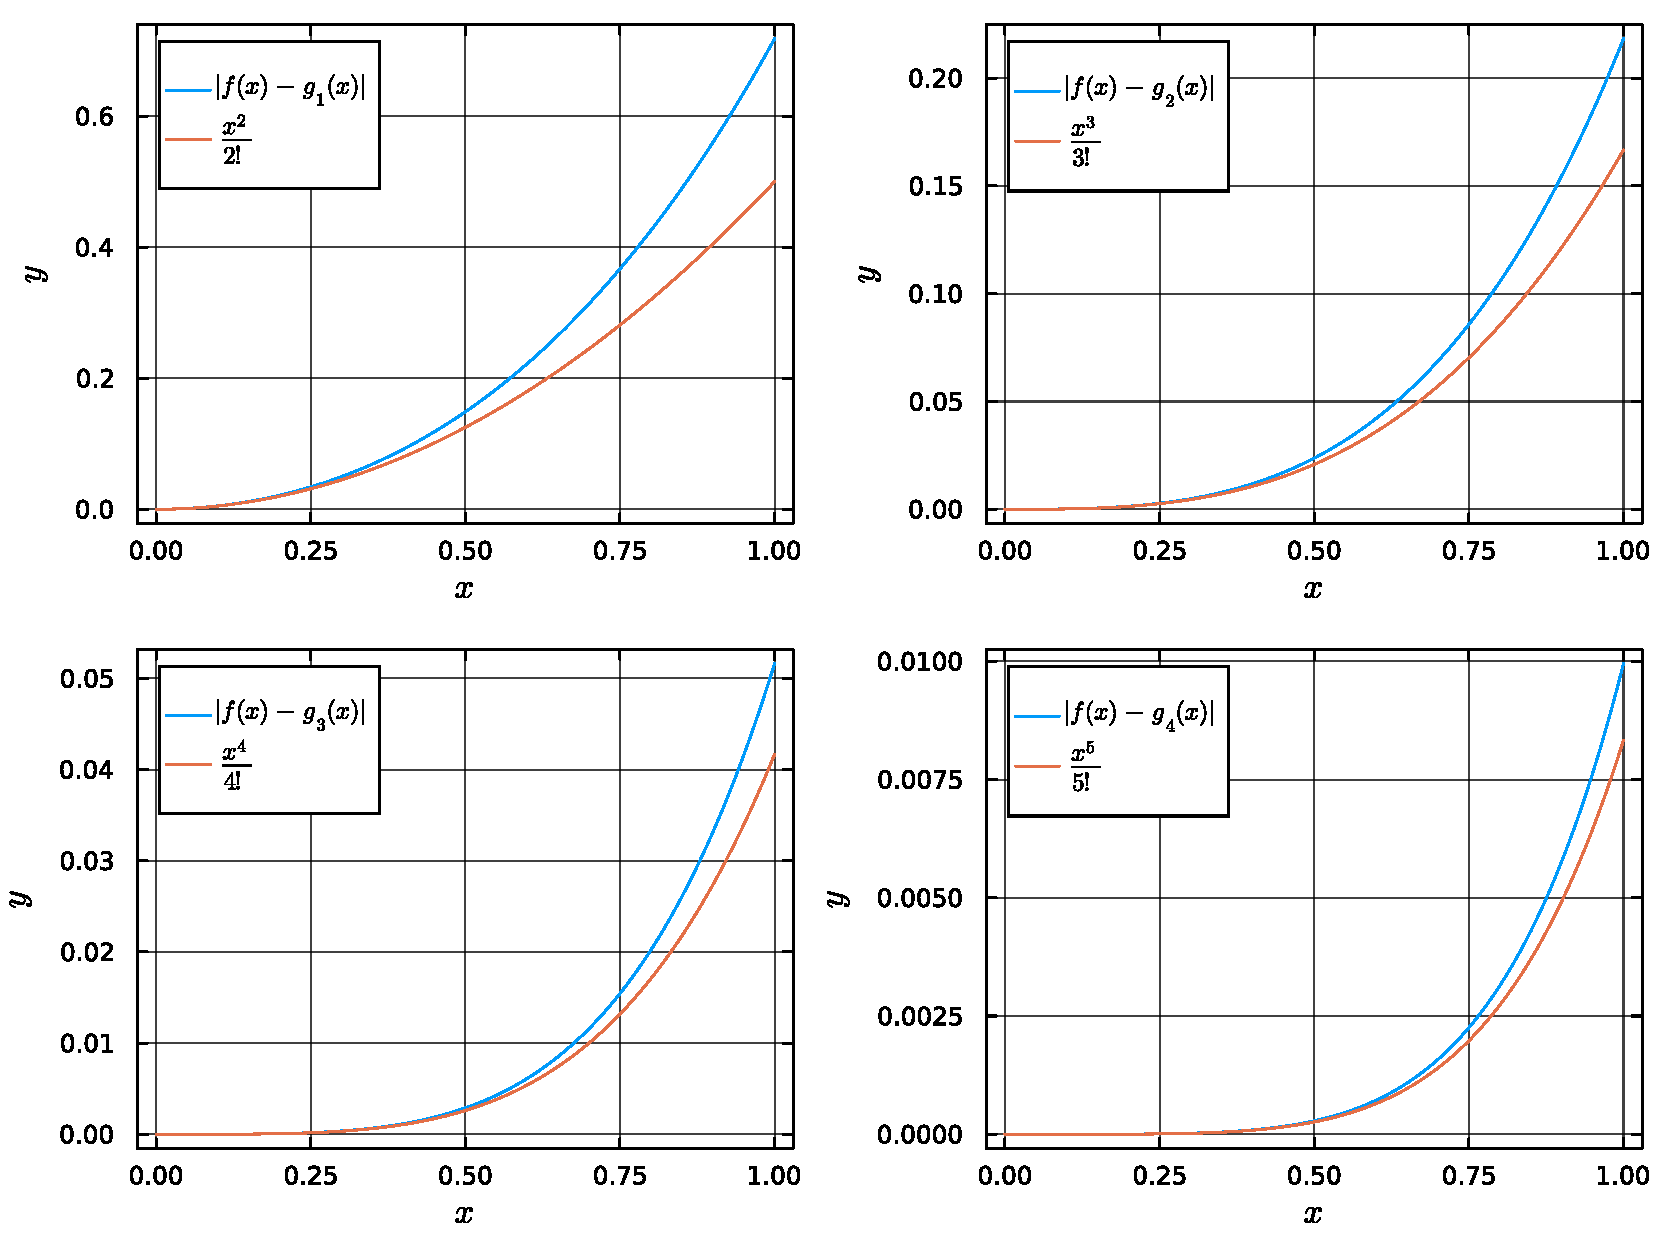
\includegraphics[width=0.8\textwidth]{1011.pdf}
    \caption{Confronto tra $\Delta$ e $\frac{x^{N+1}}{(N+1)!}$ per $N=1,2,3, 4$.}
    \label{fig:es1_0_1_1}
\end{figure}

La prima considerazione che possiamo fare è che all'aumentare di $N$ la funzione $\Delta$ 
assume valori sempre più vicini allo zero. Questo significa che la distanza tra il valore 
della funzione $f(x)$ presa in esame e la sua espansione di Taylor troncata all'ordine 
$N$ diminuisce. In effetti ci aspettiamo che la funzione $\Delta$ sia 
esattamente zero nel caso in cui $N \rightarrow \infty$. Inoltre possiamo notare che la funzione $\Delta$, in ognuno
dei grafici, è tanto più prossima allo zero quanto più ci si avvicina all'origine, poichè l'espansione in serie 
richiede $x \rightarrow 0$.\\
La seconda considerazione è che le funzioni $\Delta$ e $\frac{x^{N+1}}{(N+1)!}$ si 
avvicinano tra loro all'aumentare di $N$. Questo risponde alla richiesta dell'esercizio, 
cioè che l'errore scali come un polinomio di ordine $N+1$. 

\subsection{Esercizio 1.2.1}
Calcolare la seguente somma

\begin{equation}
    \sum_{n=1}^\infty \frac{1}{n^2}=\frac{\pi^2}{6}
    =\lim_{N\to\infty} S(N)
    \quad
    \text{con}
    \quad
    S(N)=\sum_{n=1}^N \frac{1}{n^2}
\end{equation}

\begin{enumerate}
    \item Calcolare la somma in single precision utilizzando l'ordinamento normale,\\
    $n=1,2,3,\ldots,N$.
    \item Calcolare la somma in single precision utilizzando l'ordinamento inverso,\\
    $n=N,\ldots,2,1$.
    \item Studiare la convergenza di entrambe le implementazioni in funzione di $N$ tracciando il grafico di $|S(N)-\pi^2/6|$.
    \item Ripetere i punti da 1 a 3 utilizzando double precision.
    \item Sai spiegare cosa succede?
\end{enumerate}

\subsubsection{Soluzione}
Procediamo prendendo in esame i due casi, single precision e double precision.

\paragraph{Single precision:} 

Si riportano in figura \ref{fig:es1_2_1_1} gli errori di troncamento della serie 
$\sum_{n=1}^\infty \frac{1}{n^2}$, laddove $N$ è il troncamento. La somme sono state eseguite
con variabili di tipo Float32 (single precision).

\begin{figure}[!ht]
    \centering
    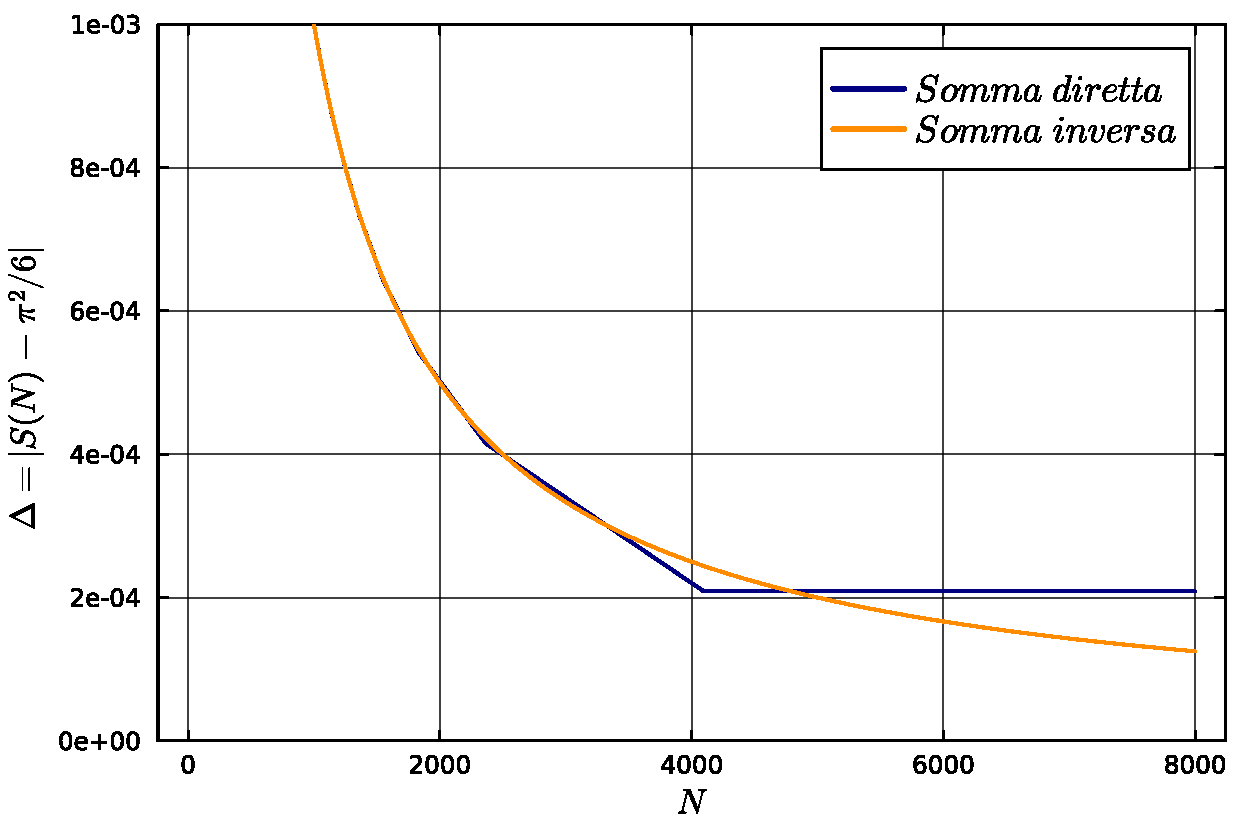
\includegraphics[width=0.8\textwidth]{1211.pdf}
    \caption{$S(N)=\sum_{n=1}^N \frac{1}{n^2}$ in single precision}
    \label{fig:es1_2_1_1}
\end{figure}

In figura \ref{fig:es1_2_1_1} notiamo due comportamenti degni di nota. Il primo riguarda
la curva blu, che arresta la sua discesa poco dopo $N = 4000$. 
Il secondo riguarda il discostarsi delle due curve, già a partire da 
$N \simeq 2000$, a causa dell'andamento a linea spezzata della curva blu.\\
La spiegazione del primo fenomeno è la seguente: nel caso della somma con ordinamento
diretto, all'aumento dell'indice di somma, gli addendi sono sempre più piccoli. In
particolare la somma comincia da 1, e sappiamo che dovrà raggiungere $\frac{\pi^2}{6} \simeq 1.64$ e perciò 
per tutto il processo la somma parziale resterà nell'intervallo $[1, 2)$. In tale intervallo la distanza tra due 
floating point numbers è $\epsilon_{mach} = 2^{-23}$. Osserviamo il grafico \ref{fig:es1_2_1_1}: la curva blu comincia ad essere 
costante a partire da $N = 4096 = 2^{12}$. Tale numero corrisponde all'addendo $\frac{1}{N^2} = 2^{-24}$, 
che è appena più piccolo di $\epsilon_{mach}$, ovvero della distanza tra due floating point numbers in $[1, 2)$, e quindi è
come sommare $0$. \\
La spiegazione del secondo fenomeno è simile: in questo caso alla somma viene aggiunto
un addendo che è più piccolo del precedente, ma non così tanto da essere più piccolo di $\epsilon_{mach}$. In
questo modo la somma viene migliorata, ma il nuovo addendo è arrotondato rispetto al suo valore vero. Il successivo
addendo, pur essendo differente in teoria, a causa dell'arrotondamento risulta essere uguale al precedente. Ciò fa
in modo che venga sommato sempre lo stesso numero, e così l'andamento della curva blu è lineare. \\
I due fenomeni non si verificano per la somma con ordinamento inverso perchè il primo numero ad essere sommato 
è molto piccolo. Questo fa in modo che i successivi floating point number siano molto vicini tra loro, è così sommare
l'addendo successivo fa cadere la somma parziale vicina al floating point number che la approssima. \\
\\
Si può mostrare matematicamente che gli errori $\Delta = |S(N)-\pi^2/6|$ scalano come $O(\frac{1}{N})$. Per verificare questa
affermazione possiamo interpolare la curva degli errori con un metodo che vedremo nella sezione \ref{sistemi_lineari}.
Sulla base delle considerazioni di questa sezione, possiamo aspettarci che sia più conveniente interpolare la curva 
con ordinamento inverso, perchè i valori che la compongono sono meno affetti da errori di tipo numerico. Utilizzando 
il modello linearizzato $log(\Delta) = -c*log(N)$ con $c = 1$ si ottiene per l'ordinamento inverso 
$c_{fit} = 1.00003$ e per quello diretto $c_{fit} = 0.986$. Come atteso il caso di ordinamento diretto restituisce un
risultato peggiore di quello inverso.


\paragraph{Double precision:}

Si riporta in figura \ref{fig:es1_2_1_2} un ingrandimento del grafico degli errori di troncamento della serie 
$\sum_{n=1}^\infty \frac{1}{n^2}$, laddove $N$ è il troncamento. La somme sono state eseguite
con variabili di tipo Float64 (double precision).

\begin{figure}[!ht]
    \centering
    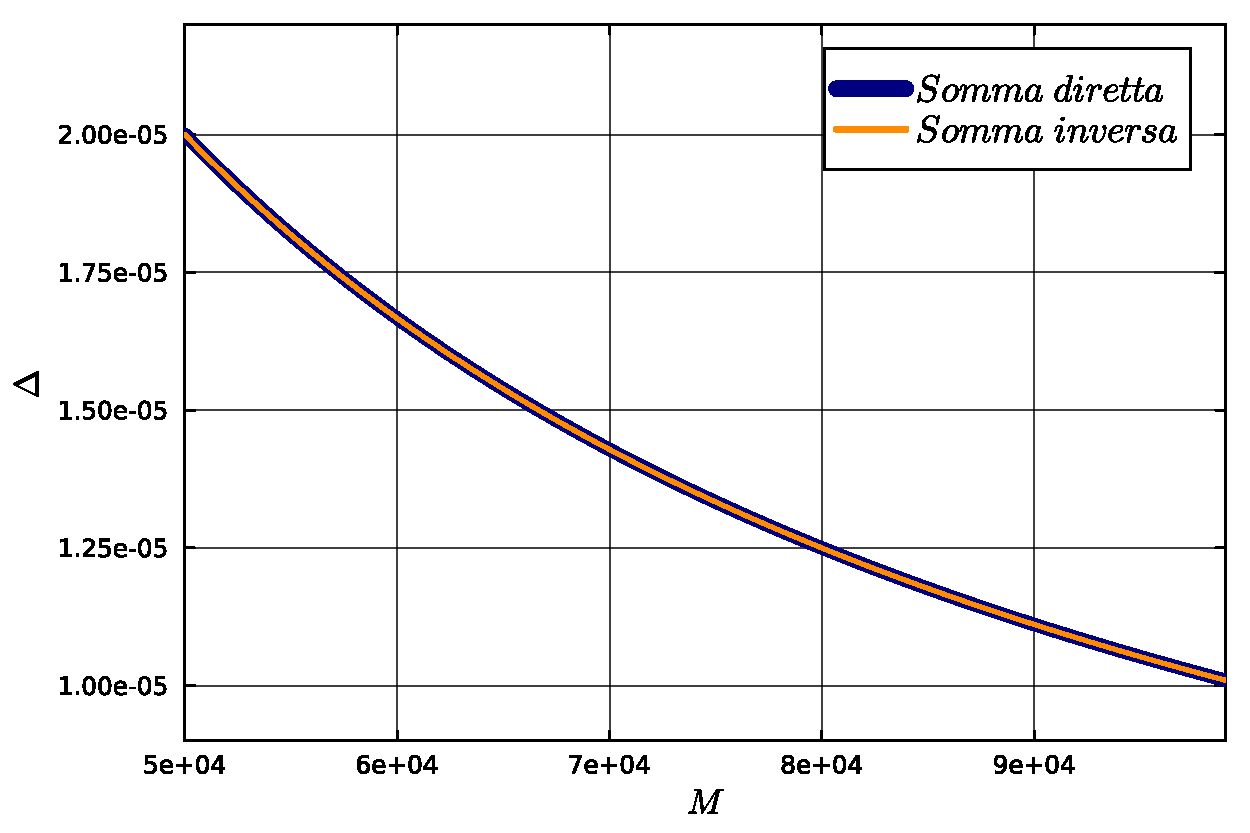
\includegraphics[width=0.8\textwidth]{1212.pdf}
    \caption{Ingrandimento di $S(N)=\sum_{n=1}^N \frac{1}{n^2}$ in double precision}
    \label{fig:es1_2_1_2}
\end{figure}

Nel caso di figura \ref{fig:es1_2_1_2} possiamo notare che le due curve sono sovrapposte, nonostante l'ingrandimento a 
valori di $N \in [5000, 10000]$. Per osservare un fenomeno simile a quello di 
figura \ref{fig:es1_2_1_1} dovremmo raggiungere valori di $N = 2^{26}$. Infatti l'approssimazione non migliora
quando vengono sommati numeri dell'ordine di $\epsilon_{mach}$ per double precision, cioè
 $\frac{1}{N^2} \simeq 2^{-52}$.

\subsection{Esercizio 1.4.1}
\paragraph{(a)} In statistica, definiamo la varianza di un campione di valori $x_1,\ldots,x_n$ come

\begin{equation}
    \sigma^2 = \frac{1}{n-1} \sum_{i=1}^n (x_i - \overline{x})^2,
    \qquad 
    \overline{x} = \frac{1}{n} \sum_{i=1}^n x_i.
    \label{eq:varianza_naive}
\end{equation}

Scrivi una funzione che prenda in input un vettore $x$ di lunghezza arbitraria e restituisca $\sigma^2$ calcolata 
con la formula sopra. 
Dovresti testare la funzione con $x=[1,1,\ldots,1]$ e con alcuni vettori casuali.

\paragraph{(b)} Uno svantaggio della formula "naive" è che bisogna prima calcolare una somma per $\overline{x}$ prima di eseguire la somma per calcolare $\sigma^2$. 
Questo significa che bisogna scorrere due volte i dati. 
Ciò è indesiderabile per grandi insiemi di dati o quando la varianza campionaria deve essere calcolata mentre i dati vengono generati. 
Alcuni libri di testo riportano una formula a singolo ciclo:

\begin{equation}
    \sigma^2 = \frac{1}{n-1} \left( u - \frac{1}{n}v^2 \right),\\
    u  = \sum_{i=1}^n x_i^2, 
    \qquad
    v = \sum_{i=1}^n x_i.  
    \label{eq:varianza_eff}  
\end{equation}

Prova entrambe le formule per i seguenti dataset, ciascuno dei quali ha varianza esattamente uguale a 1. 
Esegui i calcoli sia in single che in double precision. \\
$ x_1 = [ 1e3, 1+1e3, 2+1e3 ]$ \\
$ x_2 = [ 1e6, 1+1e6, 2+1e6 ]$ \\
$ x_3 = [ 1e7, 1+1e7, 2+1e7 ]$ \\
$ x_4 = [ 1e8, 1+1e8, 2+1e8 ]$ 

Sai spiegare i risultati?

\subsubsection{Soluzione}
\paragraph{(a) } Si è testato il codice che implementa la formula \ref{eq:varianza_naive} su tre vettori contenenti
elementi di tipo Float64. Il primo contiene solo numeri $1$, il secondo contiene numeri generati a partire 
da una distribuzione uniforme, il terzo numeri generati a partiere da una distribuzione normale. I valori sono 
riportati in tabella \ref{tab:varianza_test}.

\begin{table}[h!]
\centering
\caption{Risultati del test della formula \ref{eq:varianza_naive} su tre vettori di tipo Float64}
\label{tab:varianza_test}
\begin{tabular}{|l|c|c|c|}
\hline
\textbf{Vettore} & \textbf{Lunghezza}   & \textbf{Varianza attesa} & \textbf{Varianza (output)} \\
\hline
Solo uno         & $10^3$               & 0.000                    & 0.000                       \\
Uniforme         & $10^8$               & 0.083                    & 0.083                       \\
Normale          & $10^8$               & 1.000                    & 1.000                       \\
\hline
\end{tabular}
\end{table}

I risultati di tabella \ref{tab:varianza_test} mostrano che l'implementazione del codice è corretta.

\paragraph{(b) }
Si è testato il codice che implementa la formula \ref{eq:varianza_eff} su quattro vettori contenenti
elementi di tipo Float32, Float64 e Long Double. I risultati sono riportati in tabella \ref{tab:varianza_precisioni}.

\begin{table}[h!]
\centering
\caption{Valori di varianza. Metodo 1: equazione \ref{eq:varianza_naive}. Metodo 2: equazione \ref{eq:varianza_eff}.}
\label{tab:varianza_precisioni}
\begin{tabular}{|l|c|cc|cc|cc|}
\hline
\textbf{Set} & \textbf{$\sigma^2$ attesa} 
& \multicolumn{2}{c|}{\textbf{Float32}} 
& \multicolumn{2}{c|}{\textbf{Float64}} 
& \multicolumn{2}{c|}{\textbf{Long Double}} \\
\cline{3-8}
      &     & Metodo 1 & Metodo 2  & Metodo 1 & Metodo 2 & Metodo 1 & Metodo 2 \\
\hline
$x_1$ & 1.0 & 1.0      & 1.0       & 1.0      & 1.0      & 1.0      & 1.0 \\
$x_2$ & 1.0 & 1.0      & -131072.0 & 1.0      & 1.0      & 1.0      & 1.0 \\
$x_3$ & 1.0 & 1.0      & 0.0       & 1.0      & 1.0      & 1.0      & 1.0 \\
$x_4$ & 1.0 & 0.0      & 0.0       & 1.0      & 0.0      & 1.0      & 1.0 \\
\hline
\end{tabular}
\end{table}

I risultati di tabella \ref{tab:varianza_precisioni} mostrano che il calcolo della varianza con la formula 
\ref{eq:varianza_eff} è più affetto dalla mancanza di precisione della rappresentazione dei numeri durante il calcolo.
Infatti, mano a mano che la la precisione dei numeri aumenta, il risultato della formula \ref{eq:varianza_eff} 
si avvicina a quello atteso. \\
C'è da notare che anche la formula \ref{eq:varianza_naive} è affetta dalla stessa problematica, ma in maniera meno
evidente. Basti osservare il risultato del metodo 1 per il vettore $x_4$ in Float32, che è $0.0$, contro l'atteso 
$1.0$. \\
Parte del problema risiede nella cancellazione numerica. Infatti, per valori degli elementi del vettore molto grandi,
la differenza tra il quadrato della sommma e la somma dei quadrati è molto piccola e incorre in problema di
cancellazione. Per verificare questa affermazione, si riportano in tabella \ref{tab:errore_varianza} i valori della 
differenza \( u - \frac{v^2}{n} \)
per la formula \ref{eq:varianza_eff}.

\begin{table}[h!]
\centering
\caption{Differenza \( u - \frac{v^2}{n} \) per ciascun dataset.}
\label{tab:errore_varianza}
\begin{tabular}{|l|c|c|c|}
\hline
\textbf{Dataset} & \textbf{Single} & \textbf{Double} & \textbf{Long Double} \\
\hline
$x_1$ & 2.0       & 2.0 & 2.0 \\
$x_2$ & -262144.0 & 2.0 & 2.0 \\
$x_3$ & 0.0       & 2.0 & 2.0 \\
$x_4$ & 0.0       & 0.0 & 2.0 \\
\hline
\end{tabular}
\end{table}

Leggendo la tabella \ref{tab:errore_varianza} possiamo notare che per il dataset $x_1$ la differenza è esattamente
$2.0$, che è il risultato atteso. Per il dataset $x_2$ la differenza è molto grande, $-262144.0$, il che indica un
significativo problema di cancellazione numerica. Per il dataset $x_3$ e $x_4$, la differenza è $0.0$, indice 
del fatto che i singoli valori \( u - \frac{v^2}{n} \) sono vicini tra loro meno di $\epsilon_mach$, e perciò la 
loro differenza è zero. \\
Per concludere, possiamo dire che la formula \ref{eq:varianza_eff} è più efficiente in termini di tempo di calcolo,
ma è più affetta da errori numerici rispetto alla formula \ref{eq:varianza_naive}.

\subsection{Esercizio 1.4.2}
Sia $f(x) = \frac{e^x-1}{x}$.
  
(a) Trova il numero di condizionamento $\kappa_f(x)$. Qual è il massimo di $\kappa_f(x)$ nell'intervallo $-1\le x \le 1$?
  
(b) Usa l'algoritmo "naive"

\begin{equation}
    f(x)= \frac{e^x-1}{x}
    \label{eq:algoritmo_naive}
\end{equation}

per calcolare $f(x)$ per $x=10^{-3},10^{-4},10^{-5},\ldots,10^{-16}$.

(c) Crea un secondo algoritmo utilizzando i primi $n$ termini della serie di Maclaurin, cioè

\begin{equation}
    p(x) = 1 + \frac{1}{2!}x + \frac{1}{3!}x^2 + \cdots + \frac{1}{(n+1)!}x^n.
    \label{eq:algoritmo_maclaurin}
\end{equation}

Valutalo sugli stessi valori di $x$ del punto (b). Per farlo devi scegliere un valore per $n$. Verifica la stabilità del risultato al variare di $n$. Avresti potuto indovinare un buon valore di $n$ fin dall'inizio?

(d) Confronta i risultati delle due implementazioni in funzione di $x$. Quale algoritmo pensi sia più accurato, e perché?

\subsubsection{Soluzione}

\paragraph{(a) } Il numero di condizionamento di una funzione $f$ è definito come:
\begin{equation}
    \kappa_f(x) = \left| \frac{x f'(x)}{f(x)} \right|\,.
\end{equation}

Per la funzione $f(x) = \frac{e^x-1}{x}$, calcoliamo la derivata:
\begin{equation}
    f'(x) = \frac{e^x x - (e^x - 1)}{x^2} = \frac{e^x (x-1) + 1}{x^2}\,.
\end{equation}
Quindi il numero di condizionamento diventa:
\begin{equation}
    \kappa_f(x) = \left| \frac{x \left( \frac{e^x (x-1) + 1}{x^2} \right)}{\frac{e^x - 1}{x}} \right| = \left| \frac{e^x (x-1) + 1}{(e^x - 1)x} \right| = \left| \frac{e^x x}{(e^x - 1)} - 1 \right|\,.
\end{equation}
La derivata di $k_f(x)$ non si annulla mai nell'intervallo $-1 \leq x \leq 1$, e $\kappa_f(0) = 0$. Dato che
$\kappa_f(x)$ è monotona crescente per $x \geq 0$ e monotona decrescente per $x < 0$, il massimo si ha in $x = 1$,
dove assume il valore $\kappa_f(1) = 0.58198$.

\paragraph{(b)-(c): } Si riportano in figura \ref{fig:es1_4_2_1} i risultati dei due algoritmi. La dicitura $f(x)$ 
si riferisce alla funzione calcolata con l'algoritmo "naive", mentre $p_n(x)$ si riferisce alla funzione calcolata 
con la serie di Maclaurin, fino al termine $n$.

\begin{figure}[!ht]
    \centering
    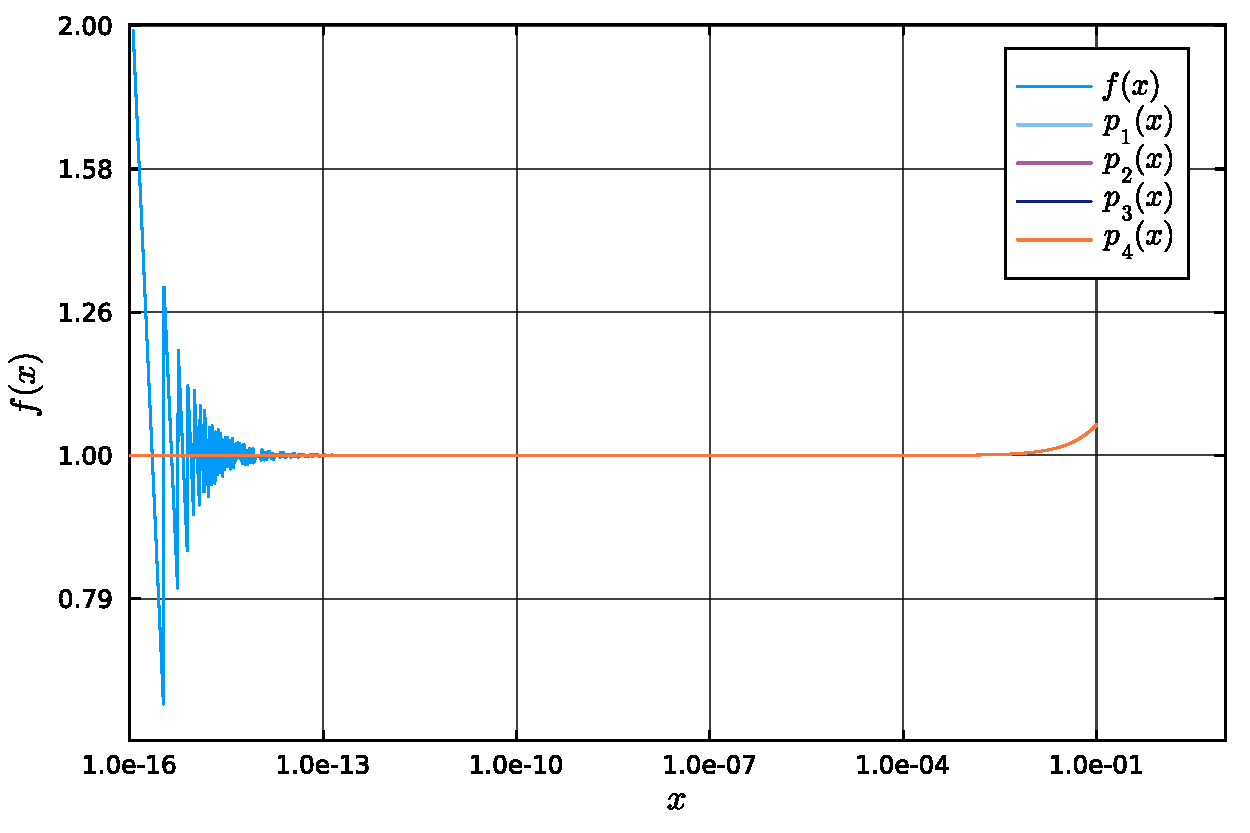
\includegraphics[width=0.8\textwidth]{1421.pdf}
    \caption{Confronto tra $f(x)$ e $p_n(x)$ al variare di $x$.}
    \label{fig:es1_4_2_1}
\end{figure}

Per uno studio più accurato, si riporta in figura \ref{fig:es1_4_2_2} un ingrandimento per piccoli valori di x 
(range $[10^{-15}, 10^{-14}]$) della figura \ref{fig:es1_4_2_1} e in figura \ref{fig:es1_4_2_3} un ingrandimento 
per valori di x (range $[10^{-2}, 10^{-1}]$) della figura \ref{fig:es1_4_2_1}.
\begin{figure}[!ht]
    \centering
    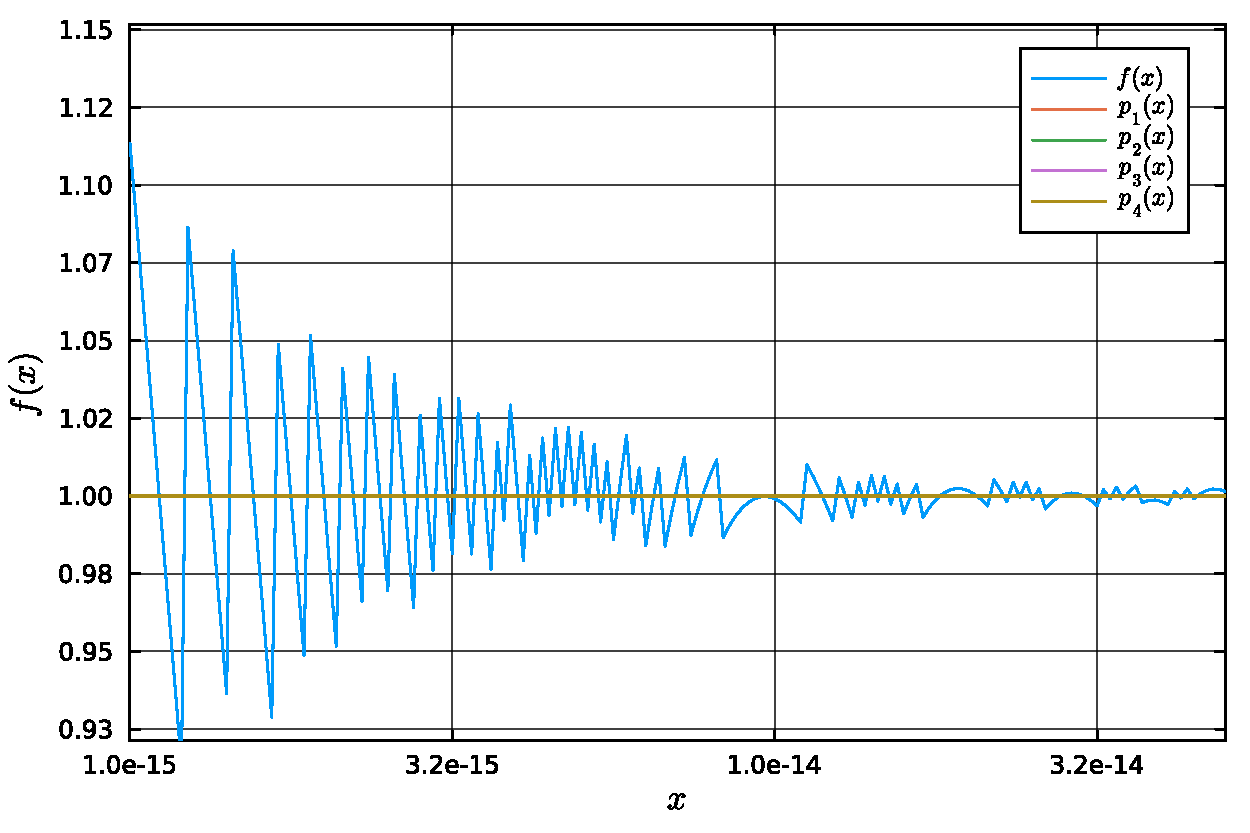
\includegraphics[width=0.8\textwidth]{1422.pdf}
    \caption{Ingrandimento di $f(x)$ e $p_n(x)$ per piccoli valori di x.}
    \label{fig:es1_4_2_2}
\end{figure}
\begin{figure}[!ht]
    \centering
    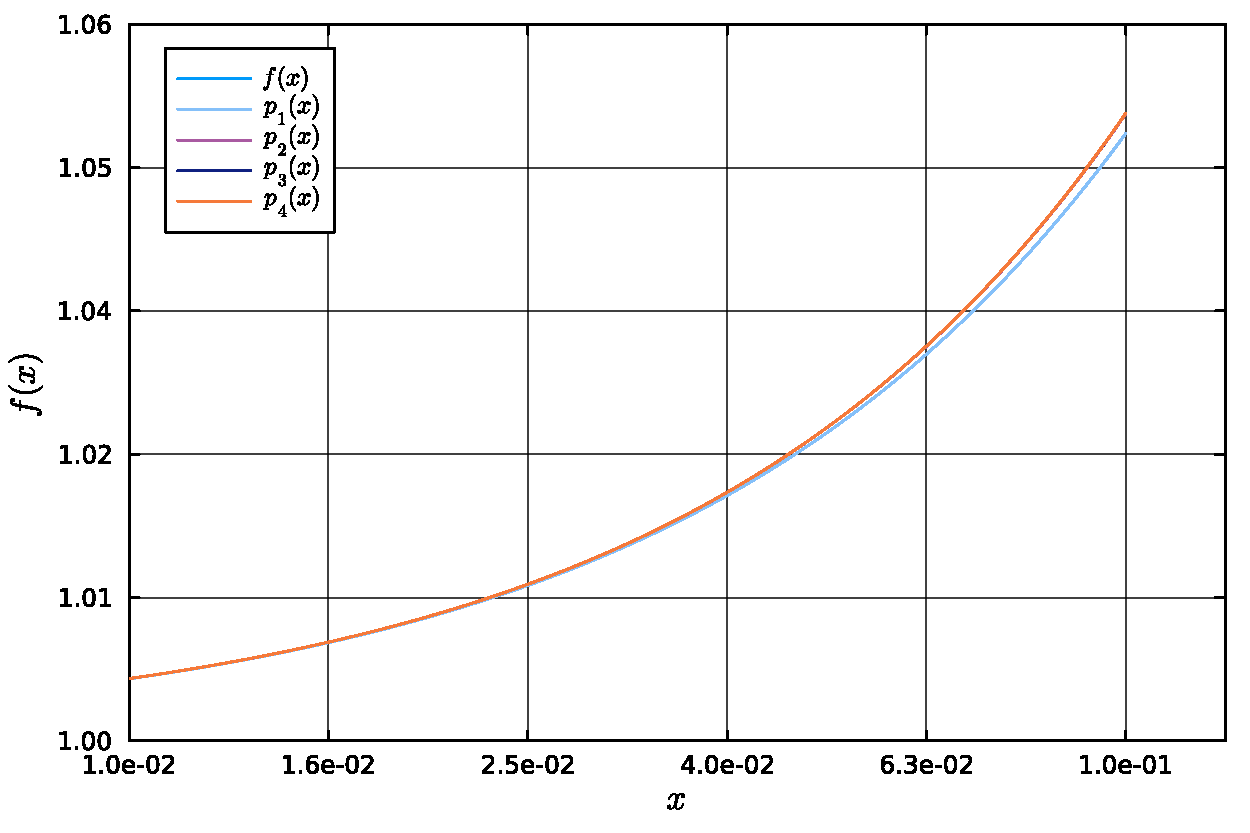
\includegraphics[width=0.8\textwidth]{1423.pdf}
    \caption{Ingrandimento di $f(x)$ e $p_n(x)$ per valori di x nell'intervallo $[10^{-2}, 10^{-1}]$.}
    \label{fig:es1_4_2_3}
\end{figure}

Per quanto riguarda il comportamento della funzione $f(x)$ calcolata con l'algoritmo \ref{eq:algoritmo_naive},
possiamo notare che per valori di $x$ piccoli, in particolare nella regione rappresentata in figura 
\ref{fig:es1_4_2_2}, la funzione assume valori non corretti, nonostante $\kappa_f(x)$ abbia un massimo non molto
grande e peraltro non assunto nell'intorno di zero. La spiegazione di questo fenomeno è che l'algoritmo
\ref{eq:algoritmo_naive}, nonostante non abbia $\kappa_f(x)$ complessivo molto grande, è affetto da errori 
di cancellazione numerica a causa della forma in cui è scritta la funzione, ma non a causa del fatto che 
il problema sia intrinsecamente instabile. Di fatto possiamo intuire che esista una possibile riscrittura
della funzione che non sia affetta da cancellazione numerica, e che sia più stabile, proprio perchè 
sappiamo che il massimo di $\kappa_f(x)$ non è molto grande. Tale riscrittura è quella che utilizza la
serie di Maclaurin, implementata nell'algoritmo $p_n(x)$. \\
Possiamo notare che l'algoritmo \ref{eq:algoritmo_maclaurin}, per valori di $x$ piccoli, restituisce il 
valore corretto, dato che non è affetto da cancellazione numerica. Al contrario, nella regione ingradita di 
figura \ref{fig:es1_4_2_3}, l'algoritmo \ref{eq:algoritmo_maclaurin} comincia a restituire valori errati
perchè ci allontaniamo dalla regione di convergenza della serie di Maclaurin. \\
Osservando la figura \ref{fig:es1_4_2_3}, notiamo che, per valori di $x$ fissati, l'algoritmo 
\ref{eq:algoritmo_maclaurin} è stabile, cioè le curve che descrivono i valori di $p_n(x)$ sono sempre più 
vicine tra loro all'aumentare di $n$, fino a sovrapporsi. Per stimare un buon valore di $n$ da utilizzare
per calcolare $p_n(x)$, possiamo osservare che la serie di Maclaurin è tanto meno stabile quanto più ci si
allontana da zero. Nel caso di studio valutiamo la distanza tra i valori di $p_n(x)$ al variare di $n$,
fissato $x = 0.1$. Si è rappresentato in figura \ref{fig:es1_4_2_4} l'andamento della distanza tra i valori
di $p_n(0.1)$ e $p_{n+1}(0.1)$ al variare di $n$. In formula:
\begin{equation}
    \Delta_n = |p_n(0.1) - p_{n+1}(0.1)|\,.
\end{equation}
\begin{figure}[!ht]
    \centering
    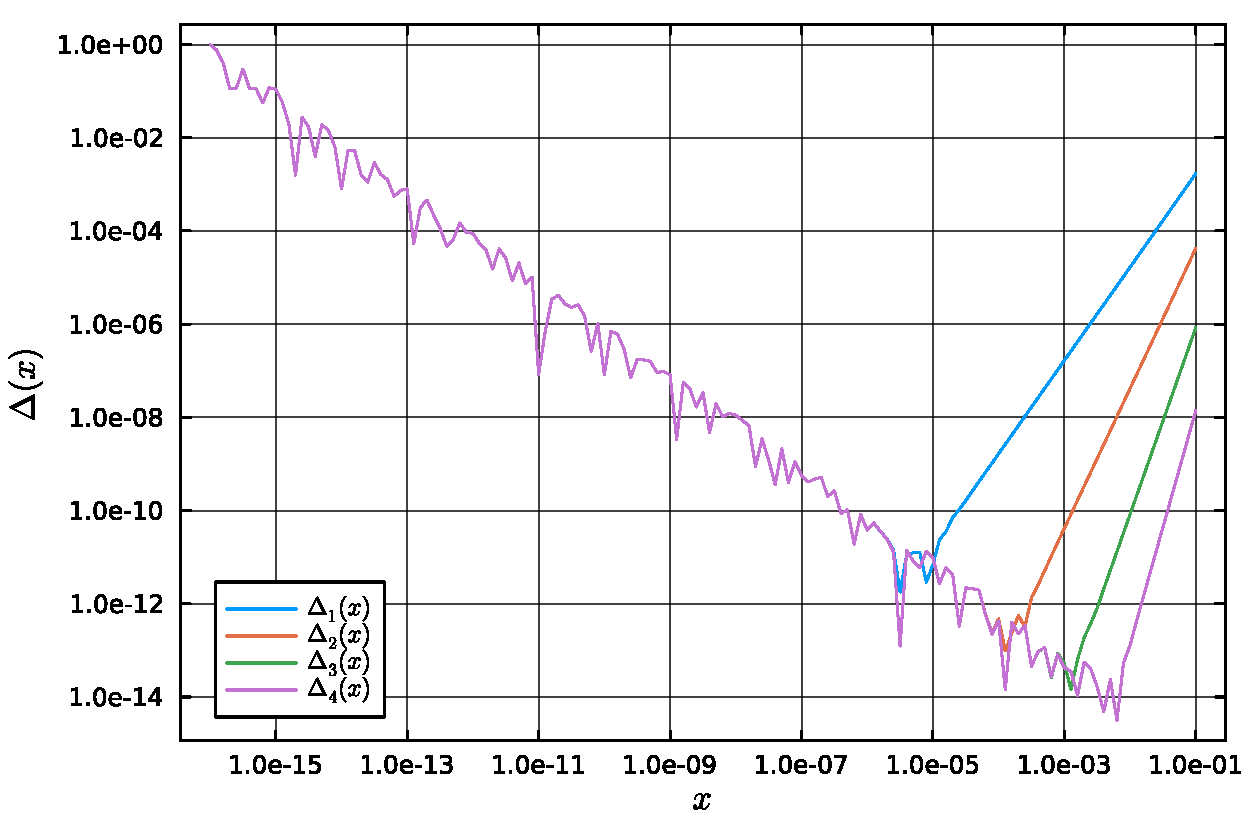
\includegraphics[width=0.8\textwidth]{1424.pdf}
    \caption{Distanza tra $p_n(0.1)$ e $p_{n+1}(0.1)$ al variare di $n$.}
    \label{fig:es1_4_2_4}
\end{figure}

Ai fini di questo esercizio possiamo dire che $n = 2$ è già un buon valore perchè le distanze tra i 
polinomi successivi non sono apprezzabili nel range $[1, 1.06]$, caratteristico della figura \ref{fig:es1_4_2_3}.
È chiaro che volendo raggiungere precisione massima occorrerà scegliere $n = 10$, dato che $\Delta_n$ 
corrispondente è più piccolo di $\epsilon{mach}$

\paragraph{(d): } Come confronto tra i due algoritmi si riporta in figura \ref{fig:es1_4_2_4} il grafico 
dell'errore tra i due algoritmi, cioè
\begin{equation}
    \Delta(x) = \left| f(x) - p_n(x) \right|\,.
\end{equation}

\begin{figure}[!ht]
    \centering
    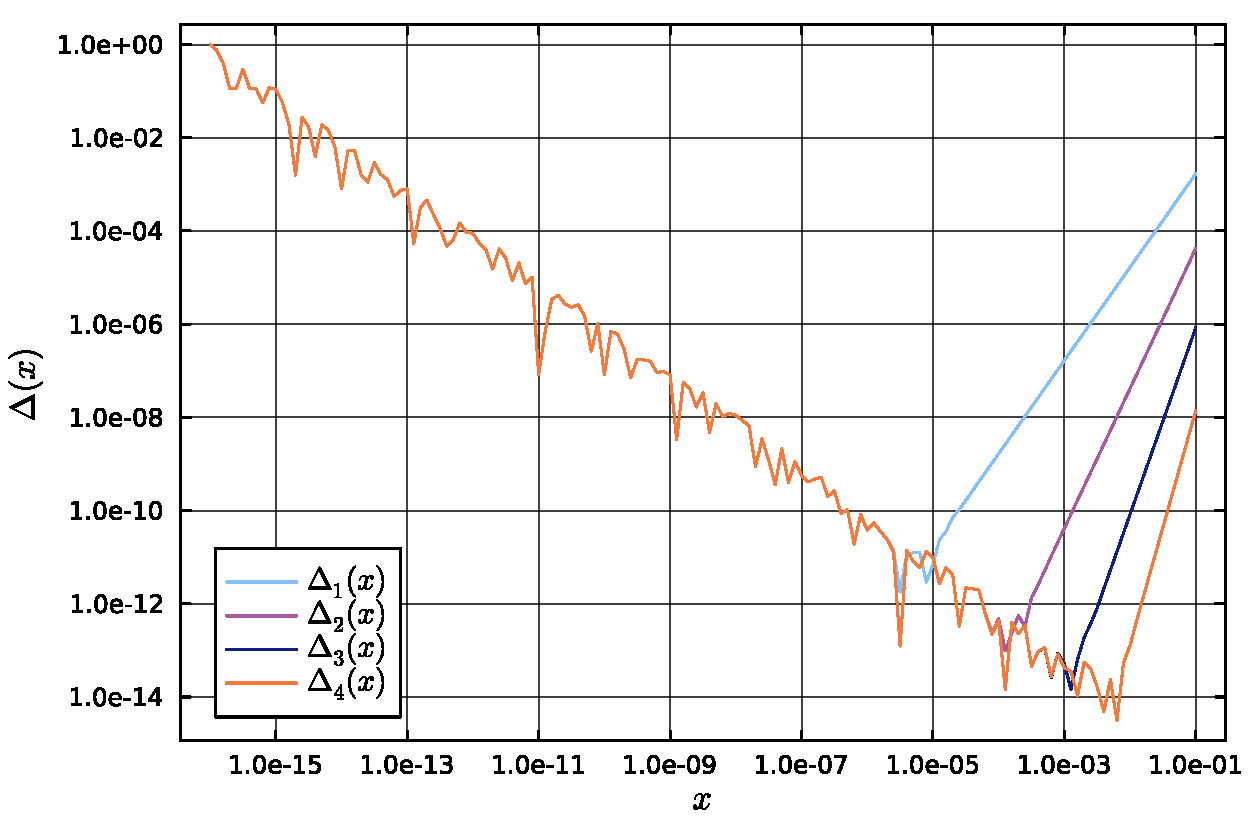
\includegraphics[width=0.8\textwidth]{1425.pdf}
    \caption{Distanza tra $f(x)$ e $p_n(x)$.}
    \label{fig:es1_4_2_5}
\end{figure}

La figura \ref{fig:es1_4_2_5} mostra una evidente differenza tra i due algoritmi nella regione di instabilità
numerica di dell'algoritmo \ref{eq:algoritmo_naive}, cioè per valori di $x$ piccoli. E' interessante notare che 
la distanza tra i due algoritmi diminuisce all'aumentare di $x$, ma torna ad aumentare a partire da
$x = 10^{-5}$, laddove l'algoritmo \ref{eq:algoritmo_maclaurin} esce dalla regione di convergenza della 
serie di Maclaurin. \\
In conclusione, possiamo affermare che l'algoritmo \ref{eq:algoritmo_maclaurin} è più accurato
per valori di $x$ piccoli, mentre l'algoritmo \ref{eq:algoritmo_naive} è più accurato per valori di $x$
grandi.

\section{Sistemi lineari}
\label{sistemi_lineari}
\subsection{Teoria}

\subsection{Esercizi 2.1.1, 2.1.2, 2.1.3, 2.1.4}
Scrivi una funzione che esegua la sostituzione in avanti su una matrice triangolare inferiore $n\times n$.

2. Testa il tuo codice sui seguenti sistemi lineari:
     
    \begin{minipage}{0.48\textwidth}
        (a) $\; \begin{bmatrix}
            -2 & 0 & 0 \\
            1 & -1 & 0 \\
            3 & 2 & 1 
          \end{bmatrix} 
          \mathbf{x} = \begin{bmatrix}
            -4 \\ 2 \\ 1
          \end{bmatrix}$
    \end{minipage}
    \hfill
    \begin{minipage}{0.48\textwidth}
        (b) $\;\begin{bmatrix}
            4 & 0 & 0 & 0 \\
            1 & -2 & 0 & 0 \\
            -1 & 4 & 4 & 0 \\
            2 & -5 & 5 & 1
          \end{bmatrix} 
          \mathbf{x} = \begin{bmatrix}
            -4 \\ 1 \\ -3 \\ 5
          \end{bmatrix}$
    \end{minipage}

Puoi verificare la soluzione risolvendo il sistema a mano e/o calcolando $\mathbf{L}\mathbf{x} - \mathbf{b}$.

3. Scrivi una funzione che esegua la sostituzione all'indietro su una matrice triangolare superiore $n\times n$.

4. Testa il tuo codice sui seguenti sistemi lineari:

    \begin{minipage}{0.48\textwidth}
        (a) $\;\begin{bmatrix}
            3 & 1 & 0  \\
            0 & -1 & -2  \\
            0 & 0 & 3  \\
            \end{bmatrix} \mathbf{x} = \begin{bmatrix}
            1 \\ 1 \\ 6
            \end{bmatrix}$
    \end{minipage}
    \hfill
    \begin{minipage}{0.48\textwidth}
        (b) $\;\begin{bmatrix}
            3 & 1 & 0 & 6 \\
            0 & -1 & -2 & 7 \\
            0 & 0 & 3 & 4 \\
            0 & 0 & 0 & 5
            \end{bmatrix} \mathbf{x} = \begin{bmatrix}
            4 \\ 1 \\ 1 \\ 5
            \end{bmatrix}$
    \end{minipage}

Puoi verificare la soluzione risolvendo il sistema a mano e/o calcolando $\mathbf{U}\mathbf{x} - \mathbf{b}$.



\subsubsection{Soluzione}
Per risolvere i sistemi lineari proposti, si sono implementate le funzioni di sostituzione in avanti e all'indietro. 
Di seguito sono riportati i risultati delle soluzioni.
\paragraph{Sostituzione in avanti:}
\begin{itemize}
    \item Per il sistema (a) si ha $\mathbf{x} = \begin{bmatrix} -4.0 & 2.0 & 1.0 \end{bmatrix}$.
    \item Per il sistema (b) si ha $\mathbf{x} = \begin{bmatrix} -4.0 & 1.0 & -3.0 & 5.0 \end{bmatrix}$.
\end{itemize}
Risolvendo i sistemi a mano, i valori sono:
\begin{itemize}
    \item Per il sistema (a) si ha $\mathbf{x} = \begin{bmatrix} -4 & 2 & 1 \end{bmatrix}$.
    \item Per il sistema (b) si ha $\mathbf{x} = \begin{bmatrix} -4 & 1 & -3 & 5 \end{bmatrix}$.
\end{itemize}
\paragraph{Sostituzione all'indietro:}
\begin{itemize}
    \item Per il sistema (a) si ha $\mathbf{x} = \begin{bmatrix} 1.0 & 1.0 & 6.0 \end{bmatrix}$.
    \item Per il sistema (b) si ha $\mathbf{x} = \begin{bmatrix} 4.0 & 1.0 & 1.0 & 5.0 \end{bmatrix}$.
\end{itemize}
Risolvendo i sistemi a mano, i valori sono:
\begin{itemize}
    \item Per il sistema (a) si ha $\mathbf{x} = \begin{bmatrix} 1 & 1 & 6 \end{bmatrix}$.
    \item Per il sistema (b) si ha $\mathbf{x} = \begin{bmatrix} 4 & 1 & 1 & 5 \end{bmatrix}$.
\end{itemize}
I risultati confermano la correttezza delle implementazioni delle funzioni di sostituzione in avanti e all'indietro.

\subsection{Esercizi 2.3.1, 2.3.2, 2.3.4}
1. Scrivi una funzione che esegua la fattorizzazione LU di una matrice $n\times n$.

2. Per ciascuna matrice, calcola la fattorizzazione LU e verifica la correttezza.

    \begin{center}
    \begin{minipage}{0.32\textwidth}
    \centering
    (a)
    \[
    \begin{bmatrix}
    2 & 3 & 4 \\
    4 & 5 & 10 \\
    4 & 8 & 2
    \end{bmatrix}
    \]
    \end{minipage}
    \hfill
    \begin{minipage}{0.32\textwidth}
    \centering
    (b)
    \[
    \begin{bmatrix}
    6 & -2 & -4 & 4\\
    3 & -3 & -6 & 1 \\
    -12 & 8 & 21 & -8 \\
    -6 & 0 & -10 & 7
    \end{bmatrix}
    \]
    \end{minipage}
    \hfill
    \begin{minipage}{0.32\textwidth}
    \centering
    (c)
    \[
    \begin{bmatrix}
    1 & 4 & 5 & -5 \\
    -1 & 0 & -1 & -5 \\
    1 & 3 & -1 & 2 \\
    1 & -1 & 5 & -1 
    \end{bmatrix}
    \]
    \end{minipage}
    \end{center}

4. Calcola il determinante delle matrici dell'Esercizio 2 utilizzando la loro fattorizzazione LU.

\subsubsection{Soluzione}
\paragraph{(Punti 1 e 2: )} Si sono implementati gli algoritmi di fattorizzazione LU, e si sono testati 
sui tre sistemi proposti. \\
Le scomposizioni ottenute sono le seguenti: \newline
    \begin{center}
    
    \[
    \textbf{(A)    }
    \mathbf{L}_A =
    \begin{bmatrix}
    1.0  & 0.0 & 0.0 \\
    2.0  & 1.0 & 0.0 \\
    2.0  & -2.0 & 1.0
    \end{bmatrix}
    \qquad
    \mathbf{U}_A =
    \begin{bmatrix}
    2.0 &  3.0  & 4.0 \\
    0.0  & -1.0  & 2.0 \\
    0.0  & 0.0   & -2.0
    \end{bmatrix}
    \qquad
    \]

    \[
    \textbf{(B)   }
    \mathbf{L}_B =
    \begin{bmatrix}
    1.0  & 0.0   & 0.0  & 0.0 \\
    0.5  & 1.0   & 0.0  & 0.0 \\
    -2.0  & -2.0  & 1.0  & 0.0 \\
    -1.0  & 1.0   & -2.0 & 1.0 \\
    \end{bmatrix}
    \qquad
    \mathbf{U}_B =
    \begin{bmatrix}
    6.0  & -2.0  & -4.0  & 4.0  \\
    0.0  & -2.0  & -4.0  & -1.0 \\
    0.0  & 0.0   & 5.0   & -2.0 \\
    0.0  & 0.0   & 0.0   & 8.0  \\
    \end{bmatrix}
    \qquad
    \]

    \[
    \textbf{(C)   }
    \mathbf{L}_C =
    \begin{bmatrix}
    1.0  & 0.0   & 0.0  & 0.0 \\
    -1.0  & 1.0   & 0.0  & 0.0 \\
    1.0  & -0.25 & 1.0  & 0.0 \\
    1.0  & -1.25 & -1.0 & 1.0 
    \end{bmatrix}
    \qquad
    \mathbf{U}_C =
    \begin{bmatrix}
    1.0  & 4.0   & 5.0  & -5.0 \\
    0.0  & 4.0   & 4.0  & -10.0 \\
    0.0  & 0.0   & -2.0 & 6.0 \\
    0.0  & 0.0   & 0.0  & 2.0 
    \end{bmatrix}
    \qquad
    \]
    \end{center}

Per verificare la correttezza delle scomposizioni, si è calcolato il prodotto $\mathbf{L}\mathbf{U}$ per ciascuna 
matrice e lo si è sottratto alla matrice originale. Si sono ottenute matrici di zeri, in tutti i casi, 
confermando la correttezza dell'algoritmo.

\paragraph{(Punto 4: )} Si è calcolato il determinante delle matrici dell'esercizio 2 utilizzando la loro
fattorizzazione LU. Ricordando le proprietà del determinante e che la matrice $\mathbf{L}$ è triangolare inferiore 
con elementi diagonali unitari, si ha che:

\begin{equation}
    \det(M) = det(LU) = \det(\mathbf{L}) \cdot \det(\mathbf{U}) = \det(\mathbf{U})\,.
\end{equation}

Per il calcolo del determinante delle matrici proposte si è eseguito il prodotto degli elementi della diagonale
principale della matrice $\mathbf{U}$. A titolo di confronto si è calcolato il determinante delle matrici con 
la funzione \texttt{det} di Julia. I risultati sono riportati in tabella \ref{tab:determinanti}.
\begin{table}[h!]
\centering
\caption{Determinanti delle matrici dell'esercizio 2.}
\label{tab:determinanti}
\begin{tabular}{|l|c|c|}
\hline
\textbf{Matrice} & \textbf{Determinante (LU)} & \textbf{Determinante (Julia)} \\
\hline
A                & 4.0                        & 4.0 \\
B                & -480.0                     & -480.0 \\
C                & 80.0                       & 80.0  \\
\hline
\end{tabular}
\end{table}

Si ottengono risultati identici.

\subsection{Esercizio 2.3.3}
Le matrici
\[
\mathbf{T}(x,y) = \begin{bmatrix}
    1 & 0 & x \\ 
    0 & 1 & y \\ 
    0 & 0 & 1
\end{bmatrix},\qquad
\mathbf{R}(\theta) = \begin{bmatrix}
    \cos\theta & \sin \theta & 0 \\ 
    -\sin\theta & \cos \theta & 0 \\
    0 & 0 & 1
\end{bmatrix}
\]
sono usate per rappresentare traslazioni e rotazioni di punti del piano in computer grafica. Per quanto segue, sia
\[
\mathbf{A} = \mathbf{T}(3,-1)\,\mathbf{R}(\pi/5)\,\mathbf{T}(-3,1), \qquad 
\mathbf{z} = \begin{bmatrix}
    2 \\ 2 \\ 1
\end{bmatrix}.
\]

\begin{enumerate}
        \item[(a)] Calcolare $\mathbf{b} = \mathbf{A}\mathbf{z}$.
        \item[(b)] Trovare la fattorizzazione LU di $\mathbf{A}$.
        \item[(c)] Usare i fattori e le sostituzioni triangolari per risolvere $\mathbf{A}\mathbf{x} = \mathbf{b}$ 
                   e calcolare $\mathbf{x} - \mathbf{z}$.
\end{enumerate}

\subsubsection{Soluzione}
\paragraph{(a) } Si calcola il prodotto tra le matrici $\mathbf{A}$ e $\mathbf{z}$, ottenendo:
\begin{equation}
    \mathbf{b} = \mathbf{A}\mathbf{z} = \begin{bmatrix}
        3.95 \\
        2.01 \\
        1.0
    \end{bmatrix}. 
\end{equation}
\paragraph{(b) } Si calcola la fattorizzazione LU della matrice $\mathbf{A}$, ottenendo:
\begin{equation}
    \mathbf{L} = \begin{bmatrix}
        1.0  &     0.0  & 0.0 \\
        -0.8  &  1.0  & 0.0 \\
        0.0  &  0.0  &  1.0
    \end{bmatrix}, \qquad
    \mathbf{U} = \begin{bmatrix}
        0.81  &  0.59  &  1.16 \\
        0.0       &  1.24   &  2.42 \\
        0.0       &  0.0       &  1.0
    \end{bmatrix}.
\end{equation}
\paragraph{(c) } Si risolve il sistema $\mathbf{A}\mathbf{x} = \mathbf{b}$ utilizzando le sostituzioni triangolari.
Si ottiene, con le dovute approssimazioni:
\begin{equation}
    \mathbf{x} = \begin{bmatrix}
        2.0 \\ 
        2.0 \\ 
        1.0
    \end{bmatrix}.
\end{equation}
La differenza tra $\mathbf{x}$ e $\mathbf{z}$ è:
\begin{equation}
    \mathbf{x} - \mathbf{z} = \begin{bmatrix}
        -2.22 \cdot 10^{-16}  \\
        -4.44 \cdot 10^{-16}  \\
        0.0
    \end{bmatrix}.
\end{equation}

\subsection{Esercizi 2.4.1, 2.4.2}
1. Scrivi un programma che esegua la decomposizione di Cholesky di una matrice $n\times n$. \\
2. Per ciascuna matrice, utilizza la decomposizione di Cholesky per determinare se è definita positiva.

\begin{center}
    \begin{minipage}{0.32\textwidth}
    \centering
    \[
    \mathbf{A} =
    \begin{bmatrix}
    1 & 0 & -1 \\
    0 & 4 & 5 \\
    -1 & 5 & 10
    \end{bmatrix}
    \]
    \end{minipage}
    \hfill
    \begin{minipage}{0.32\textwidth}
    \centering
    \[
    \mathbf{B} =
    \begin{bmatrix}
    1 & 0 & 1 \\
    0 & 4 & 5 \\
    1 & 5 & 10
    \end{bmatrix}
    \]
    \end{minipage}
    \hfill
    \begin{minipage}{0.32\textwidth}
    \centering
    \[
    \mathbf{C} =
    \begin{bmatrix}
    1 & 0 & 1 \\
    0 & 4 & 5 \\
    1 & 5 & 1
    \end{bmatrix}
    \]
    \end{minipage}
\end{center}

\begin{center}
    \begin{minipage}{0.48\textwidth}
    \centering
    \[
    \mathbf{D} =
    \begin{bmatrix}
    6 & 2 & 1 & 0 \\
    2 & 6 & 2 & 1 \\
    1 & 2 & 5 & 2 \\
    0 & 1 & 2 & 4
    \end{bmatrix}
    \]
    \end{minipage}
    \hfill
    \begin{minipage}{0.48\textwidth}
    \centering
    \[
    \mathbf{E} =
    \begin{bmatrix}
    4 & 1 & 2 & 7 \\
    1 & 1 & 3 & 1 \\
    2 & 3 & 5 & 3 \\
    7 & 1 & 3 & 1
    \end{bmatrix}
    \]
    \end{minipage}
\end{center}

\subsubsection{Soluzione}
Si è implementato l'algoritmo di decomposizione di Cholesky, e si sono testate le matrici proposte. L'algoritmo
è giunto a conclusione per le matrici $\mathbf{A}$, $\mathbf{B}$ e $\mathbf{D}$, ma ha restituito un messaggio di
errore per le matrici $\mathbf{C}$ e $\mathbf{E}$, indicando che non sono definite positive. 
Si riportano i risultati delle decomposizioni giunte a termine, con i dovuti arrotondamenti. 

\begin{center}
    \begin{minipage}{0.32\textwidth}
    \centering
    \[
    \mathbf{R_A} =
    \begin{bmatrix}
        1.0  &  0.0  &  -1.0 \\
        0.0  &  2.0  &  2.5 \\
        0.0  &  0.0  &  1.7
    \end{bmatrix}
    \]
    \end{minipage}
    \hfill
    \begin{minipage}{0.32\textwidth}
    \centering
    \[
    \mathbf{R_B} =
    \begin{bmatrix}
    1.0  &  0.0  &  1.0 \\
    0.0  &  2.0  &  2.5 \\
    0.0  &  0.0  &  1.7
    \end{bmatrix}
    \]
    \end{minipage}
    \hfill
    \begin{minipage}{0.32\textwidth}
    \centering
    \[
    \mathbf{R_D} =
    \begin{bmatrix}
    2.45 & 0.82 & 0.41 & 0.00 \\
    0.00 & 2.29 & 0.73 & 0.41 \\
    0.00 & 0.00 & 2.06 & 0.82 \\
    0.00 & 0.00 & 0.00 & 1.84
    \end{bmatrix}
    \]
    \end{minipage}
\end{center}

\subsection{Esercizio 2.5.1}
Consideriamo la matrice:
\[
\mathbf{A} =
\begin{bmatrix}
-\epsilon &  1 \\
        1 & -1
\end{bmatrix}
\]

Se $\epsilon=0$, la fattorizzazione LU senza pivoting parziale fallisce per $\mathbf{A}$. Ma se $\epsilon\neq 0$, 
possiamo procedere senza pivoting, almeno in linea di principio. \\
(a) Costruisci $\mathbf{b}=\mathbf{Ax}$ prendendo $\epsilon=10^{-12}$ per la matrice $\mathbf{A}$ e 
$\mathbf{x}=[1,1]$ come soluzione. \\
(b) Fattorizza la matrice usando la decomposizione LU senza pivoting e risolvi numericamente per $\mathbf{x}$. 
Quanto è accurato il risultato? \\
(c) Verifica la fattorizzazione LU calcolando $\mathbf{A}-\mathbf{LU}$. Funziona? \\
(d) Ripeti per $\epsilon=10^{-20}$. Quanto è accurato ora il risultato? \\
(e) Calcola il numero di condizionamento della matrice $\mathbf{A}$; puoi scegliere la norma che preferisci. 
Il sistema $\mathbf{Ax}=\mathbf{b}$ è mal condizionato? \\
(f) Calcola le matrici $\mathbf{L}$ e $\mathbf{U}$ della fattorizzazione LU di $\mathbf{A}=\mathbf{LU}$ a mano. \\
(g) Calcola i numeri di condizionamento di $\mathbf{L}$ e $\mathbf{U}$. I sistemi triangolari 
$\mathbf{L}\mathbf{z}=\mathbf{b}$ e $\mathbf{U}\mathbf{x}=\mathbf{z}$ sono mal condizionati? \\

\subsubsection{Soluzione}
Per poter operare un confronto tra i risultati ottenuti con $\epsilon = 10^{-12}$ e $\epsilon = 10^{-20}$, si è
scelto di trattare il punto (d) insieme ai punti (a), (b) e (c). Il pedice 1 è legato al caso $\epsilon = 10^{-12}$,
il pedice 2 al caso $\epsilon = 10^{-20}$. \\

\paragraph{(a) } Si è calcolato il prodotto tra la matrice $\mathbf{A}$ e il vettore $\mathbf{x}$, ottenendo, 
a meno di arrotondamenti, i vettori:
\begin{equation}
    \mathbf{b_1} = \begin{bmatrix}
         1.0 \\
         0.0
    \end{bmatrix}.
\qquad
    \mathbf{b_2} = \begin{bmatrix}
         1.0\\
         0.0
    \end{bmatrix}.
\end{equation}

\paragraph{(b) } \label{par:fattorizzazione_LU} Si è calcolata la fattorizzazione LU della matrice $\mathbf{A}$, ottenendo:
\begin{equation}
    \mathbf{L_1} = \begin{bmatrix}
    1.0      &  0.0 \\
    -1.0 \cdot 10^{12}  &  1.0 
    \end{bmatrix}, \qquad
    \mathbf{U_1} = \begin{bmatrix}
    -1.0 \cdot 10^{-12}  &  1.0               \\
     0.0                 &  1.0 \cdot 10^{12}
    \end{bmatrix},
\end{equation}
\begin{equation}
    \mathbf{L_2} = \begin{bmatrix}
    1.0                 &  0.0 \\
    -1.0 \cdot 10^{20}  &  1.0
    \end{bmatrix}, \qquad
    \mathbf{U_2} = \begin{bmatrix}
    -1.0 \cdot 10^{-20}  &  1.0 \\
     0.0                 &  1.0 \cdot 10^{20}
    \end{bmatrix}.
\end{equation}

Si è risolto il sistema $\mathbf{Ax} = \mathbf{b}$ utilizzando le sostituzioni triangolari, ottenendo:
\begin{equation}
    \mathbf{x_1} = \begin{bmatrix}
        1.0 \\
        1.0
    \end{bmatrix}, 
    \qquad
    \mathbf{x_2} = \begin{bmatrix}
        0.0 \\
        1.0
    \end{bmatrix}.
\end{equation}

\paragraph{(c) } Si è calcolato il prodotto tra le matrici $\mathbf{L}$ e $\mathbf{U}$, in seguito lo si è 
sottratto ad $\mathbf{A}$ ottenendo:
\begin{equation}
    \mathbf{A_1} - \mathbf{(LU)_1} = \begin{bmatrix}
        0.0 & 0.0 \\
        0.0 & 0.0
    \end{bmatrix}, 
    \qquad
    \mathbf{A_2} - \mathbf{(LU)_2} = \begin{bmatrix}
        0.0 & 0.0 \\
        0.0 & 1.0
    \end{bmatrix}.
\end{equation}

È evidente che il risultato per $\epsilon = 10^{-12}$ è accurato, al contrario del risultato ottenuto per
$\epsilon = 10^{-20}$, in cui sia la soluzione che la verifica della fattorizzazione LU sono
affette da errori numerici.

\paragraph{(e) } Si è calcolato $\kappa(A)$, utilizzando sia la norma 1 che la norma infinito, ottenendo lo stesso
numero a causa della natura simmetrica della matrice $\mathbf{A}$. La formula generale per il numero di
condizionamento della matrice $\mathbf{A}$ presa in esame è $ \kappa(A) = \frac{4}{1 - \epsilon}$.
\begin{equation}
    \kappa_1(A) = \kappa_\infty(A) =  4.000000000004\,,
    \qquad
    \kappa_1(A) = \kappa_\infty(A) =  4.0\,.
\end{equation}

Come si può notare, in entrambi i casi il numero di condizionamento non è molto grande, quindi il sistema
$\mathbf{Ax} = \mathbf{b}$ non è mal condizionato. 

\paragraph{(f) } Si sono calcolate a mano le matrici $\mathbf{L}$ e $\mathbf{U}$ della fattorizzazione LU di
$\mathbf{A}$ per ciascun valore di $\epsilon$. I calcoli dettagliati sono disponibili nella cartella git
\verb|lab\computazionale1\esercizi\pen_and_paper|, il cui link è stato fornito in precedenza. Ad ogni modo le 
matrici ottenute sono già state riportate al punto \ref{par:fattorizzazione_LU}. \\

\paragraph{(g) } Si sono calcolati i numeri di condizionamento di $\mathbf{L}$ e $\mathbf{U}$, utilizzando sia 
la norma 1 che la norma infinito, ancora una volta ottenendo lo stesso numero. \\
Le forumle generali per il numero di condizionamento delle matrici $\mathbf{L}$ e $\mathbf{U}$ sono:
\begin{equation}
    \kappa_1(L) = \kappa_\infty(L) = \left(1 + \frac{1}{\epsilon}\right)^2\,,
    \qquad
    \kappa_1(U) = \kappa_\infty(U) = \frac{1}{\epsilon^2}\,.
\end{equation}

In tabella \ref{tab:LU_epsilon} sono riassunti i risultati ottenuti.

\begin{table}[h!]
\centering
\caption{Valori dei parametri \( L \) e \( U \) per diverse tolleranze \( \varepsilon \)}
\label{tab:LU_epsilon}
\begin{tabular}{|c|c|c|}
\hline
 & \( \varepsilon = 10^{-12} \) & \( \varepsilon = 10^{-20} \) \\
\hline
\( L \) & $1.0 \cdot 10^{24}$ & $1.0 \cdot 10^{40}$ \\
\( U \) & $1.0 \cdot 10^{24}$ & $1.0 \cdot 10^{40}$ \\
\hline
\end{tabular}
\end{table}

\subsubsection{Conclusioni}
L'esercizio ha mostrato come il numero di condizionamento di una matrice non sia un indicatore sufficiente per
valutare l'esattezza della risoluzione del sistema lineare associato. Infatti, sebbene il numero di condizionamento
della matrice $\mathbf{A}$ sia relativamente basso, la risoluzione del sistema richiede il calcolo delle matrici
$\mathbf{L}$ e $\mathbf{U}$, il cui numero di condizionamento potrebbe risultare elevato. È questo il caso
con $\epsilon = 10^{-20}$, in cui $\kappa(A) =  4.0$ ma $\kappa(L) = 1.0 \cdot 10^{40}$ e 
$\kappa(U) = 1.0 \cdot 10^{40}$. Dato che l'algoritmo utilizza le matrici $\mathbf{L}$ e $\mathbf{U}$ 
per risolvere il sistema è evidente che l'errore numerico aumenta a causa delle stesse.

\subsection{Esercizio 2.6.1}
(a) Scrivi un programma che prenda in input una matrice $\mathbf{A}$ e un vettore $\mathbf{b}$ e risolva 
il problema dei minimi quadrati $\text{argmin}\| \mathbf{b}- \mathbf{A} \mathbf{x}\|_2$ utilizzando la decomposizione di Cholesky.\\
(b) Per verificare il funzionamento del tuo codice, calcola la soluzione ai minimi quadrati quando
\begin{center}
    \begin{minipage}{0.48\textwidth}
    \centering
    \[
    \mathbf{A} = \begin{bmatrix}
      2 & -1 \\
      0 & 1 \\
      -2 & 2
    \end{bmatrix}, \qquad
    \mathbf{b} = \begin{bmatrix}
      1 \\ -5 \\ 6
    \end{bmatrix}
    \]
    \end{minipage}
\end{center}

\subsubsection{Soluzione}
Si è implementato l'algoritmo per il metodo dei minimi quadrati e lo si è testato sulle matrici proposte, 
ottenendo:
\begin{equation}
    \mathbf{x} = \begin{bmatrix}
        -2.0 \\
        -1.0
    \end{bmatrix}.
\end{equation}

\subsection{Esercizio 2.6.2}
Keplero ha scoperto che il periodo orbitale $\tau$ di un pianeta dipende dalla sua distanza media $R$ dal Sole 
secondo la legge $\tau = c R^{\alpha}$, dove $\alpha$ è un semplice numero razionale. \\
(a) Esegui un fit lineare ai minimi quadrati utilizzando la tabella \ref{tab:pianeti} per determinare il valore 
più probabile e semplice di $\alpha$. \\
Il risultato è in accordo con le tue aspettative? 
[Suggerimento: ricorda le leggi del moto planetario di Keplero.] \\
(b) Realizza un grafico dei dati e del risultato del fit.

\subsubsection{Soluzione}
\paragraph{(a) } Il metodo dei minimi quadrati che è stato sviluppato durante il corso è adatto a risolvere
problemi lineari, in cui le costanti che si vogliono determinare sono coefficienti lineari di funzioni dei dati.
Non è il caso del problema proposto, dato che $\alpha$ si trova ad esponente. Per risolvere la questione si 
è scelto di linearizzare il problema tramite il logaritmo naturale. In formule:
\begin{equation}
    \ln(\tau) = \ln(c) + \alpha \ln(R).
\end{equation}
Da qui in poi si è implementato il metodo dei minimi quadrati, applicando la scomposizione di Cholesky alla 
matrice $n \times n$ ottenuta dal prodotto della matrice di design e la sua trasposta. Per chiarezza si riporta
la matrice di design:
\begin{equation}
    \mathbf{A} = \begin{bmatrix}
        1 & \ln(57.59) \\
        1 & \ln(108.11) \\
        1 & \ln(149.57) \\
        1 & \ln(227.84) \\
        1 & \ln(778.14) \\
        1 & \ln(1427) \\
        1 & \ln(2870.3) \\
        1 & \ln(4499.9)
    \end{bmatrix}.
\end{equation}
La matrice di regressione è stata costruita in modo che la prima colonna fosse composta da 1, per poter calcolare
il termine noto della retta, e la seconda colonna fosse composta dai logaritmi naturali delle
distanze dei pianeti dal Sole. \\
La legge di Keplero prevista è la seguente:
\begin{equation}
    \label{eq:keplero}
    \tau = c R^{3/2}\,,
\end{equation}
dove $\alpha = 3/2$. \\
È necessario un ulteriore commento su \ref{eq:keplero}, prima di riportare i risultati. Fino ad ora abbiamo
assunto che la costante $c$ fosse indipendente dal pianeta, ma in realtà la sua espressione è:
\begin{equation}
    c = \frac{2\pi}{\sqrt{G (M+m)}}\,,
\end{equation}
dove $G$ è la costante di gravitazione universale, $M$ è la massa del Sole, $m$ è la massa del pianeta. \\
Consideriamo Giove, il pianeta più massivo di quelli presi in esame ($m \approx 1.90 \cdot 10^{27} \, \text{kg}$). Si ha:
\begin{align}
    c_1 &= \frac{2\pi}{\sqrt{G (M+m)}} = 5.47 \cdot 10^{-10} \frac{\text{sec}}{m^{3/2}} = 0.203 \frac{days}{Mkm^{3/2}}  \\
    c_2 &= \frac{2\pi}{\sqrt{G M}}   = 5.47 \cdot 10^{-10} \frac{\text{sec}}{m^{3/2}} = 0.203 \frac{days}{Mkm^{3/2}}    \\
    \frac{c_1}{c_2} &\approx 1.0
\end{align}

Possiamo quindi affermare che la costante $c$ è indipendente dalla massa del pianeta, entro la precisione 
necessaria per il nostro scopo. \\
Si è quindi calcolato il valore di $\alpha$ e della costante $c$, ottenendo:
\begin{equation}
    c = 0.206 \frac{days}{Mkm^{3/2}}
    \qquad
    \alpha = 1.499
\end{equation}
I risultati sono in accordo con quanto atteso.

\paragraph{(b) } Si riporta in figura \ref{fig:es2_6_2_1} il grafico dei dati e relativo fit.

\begin{figure}[!ht]
    \centering
    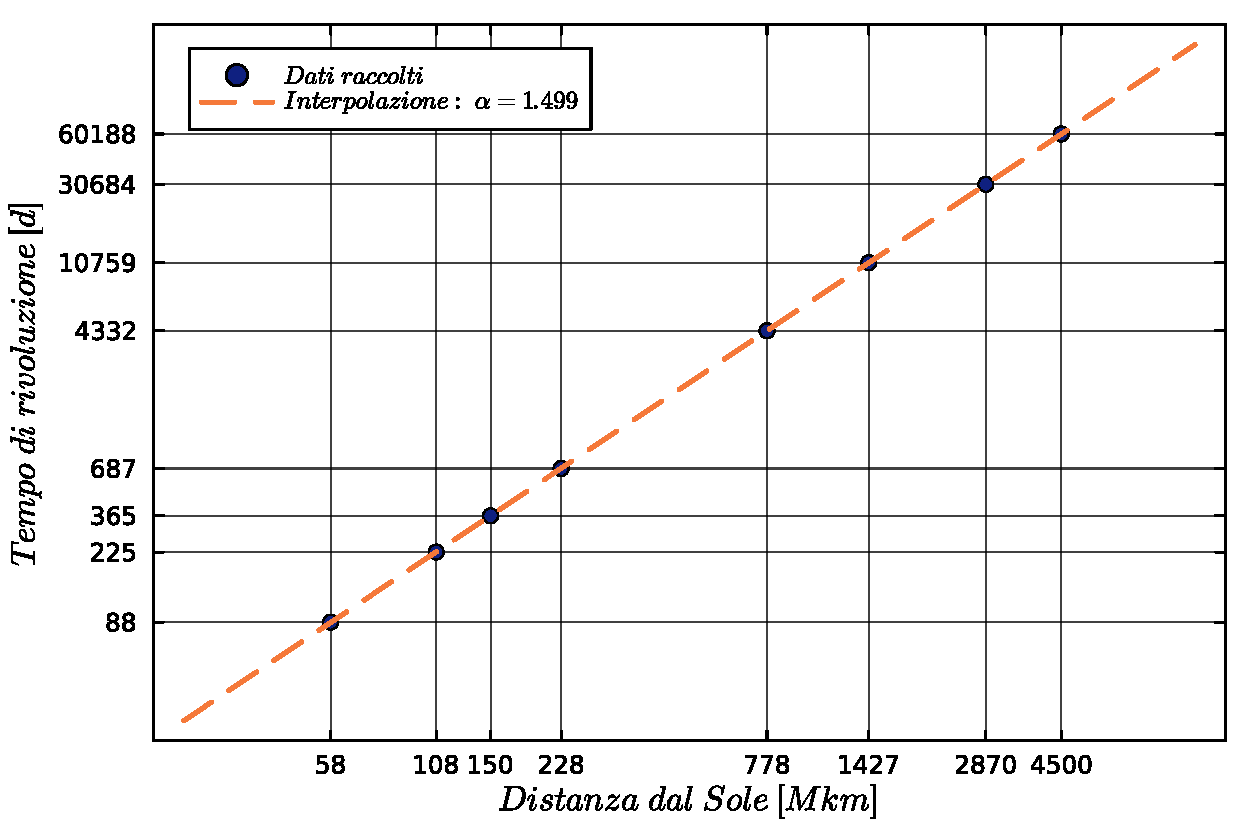
\includegraphics[width=0.8\textwidth]{2621.pdf}
    \caption{Fit lineare ai minimi quadrati dei dati dei pianeti del Sistema Solare.}
    \label{fig:es2_6_2_1}
\end{figure}

\subsection{Esercizio 2.6.3}
In questo esercizio si vuole trovare un'approssimazione della funzione periodica $g(t)=e^{\sin(t-1)}$ su un 
periodo, $0 < t \le 2\pi$. Come dati, si definiscono

\begin{equation}
    t_i = \frac{2\pi i}{60}\,,
    \quad  
    y_i = g(t_i)\,,
    \quad i=1,\ldots,60.
\end{equation}
    
(a) Trova i coefficienti del fit ai minimi quadrati    
    \begin{equation}
    \label{eq:fit_pol}    
        y(t) \approx c_1 + c_2 t + \cdots + c_7 t^6.
    \end{equation}        
Sovrapponi un grafico dei valori dei dati come punti con una curva che mostra il fit. \\
(b) Trova i coefficienti del fit ai minimi quadrati
    \begin{equation}
    \label{eq:fit_fourier}
        y \approx d_1 + d_2\cos(t) + d_3\sin(t) + d_4\cos(2t) + d_5\sin(2t).
    \end{equation}

A differenza del punto (a), questa funzione di fitting è essa stessa periodica. 
Sovrapponi un grafico dei valori dei dati come punti con una curva che mostra il fit.

\subsubsection{Soluzione}
Dopo avere generato i dati richiesti, si è eseguito il metodo dei minimi quadrati con le seguenti 
matrici di regressione:

\begin{equation}
    \mathbf{D_{pol}} = \begin{bmatrix}
        1 & t_1 & \hdots & t_1^6 \\
        1 & t_2 & \hdots & t_2^6 \\
        \vdots & \vdots & \ddots& \vdots \\
        1 & t_{60} & \hdots & t_{60}^6
    \end{bmatrix},
    \qquad
    \mathbf{D_{Four}} = \begin{bmatrix}
        1 & \cos(t_1) & \sin(t_1) & \cos(2t_1) & \sin(2t_1) \\
        1 & \cos(t_2) & \sin(t_2) & \cos(2t_2) & \sin(2t_2) \\
        \vdots & \vdots & \vdots & \vdots & \vdots \\
        1 & \cos(t_{60}) & \sin(t_{60}) & \cos(2t_{60}) & \sin(2t_{60})
    \end{bmatrix},
\end{equation}

ottenendo i coefficienti delle formule \ref{eq:fit_pol} e \ref{eq:fit_fourier}:
\begin{itemize}
    \item Coefficienti del polinomio: $[0.712; -1.351; 2.225; -0.538; -0.074; 0.033; -0.003]$
    \item Coefficienti della funzione di Fourier: $[1.266; -0.951; 0.611; 0.113; -0.247]$
\end{itemize}

Si riportano i grafici dei dati e dei fit in figura \ref{fig:es2_6_3_1}.
\begin{figure}[!ht]
    \centering
    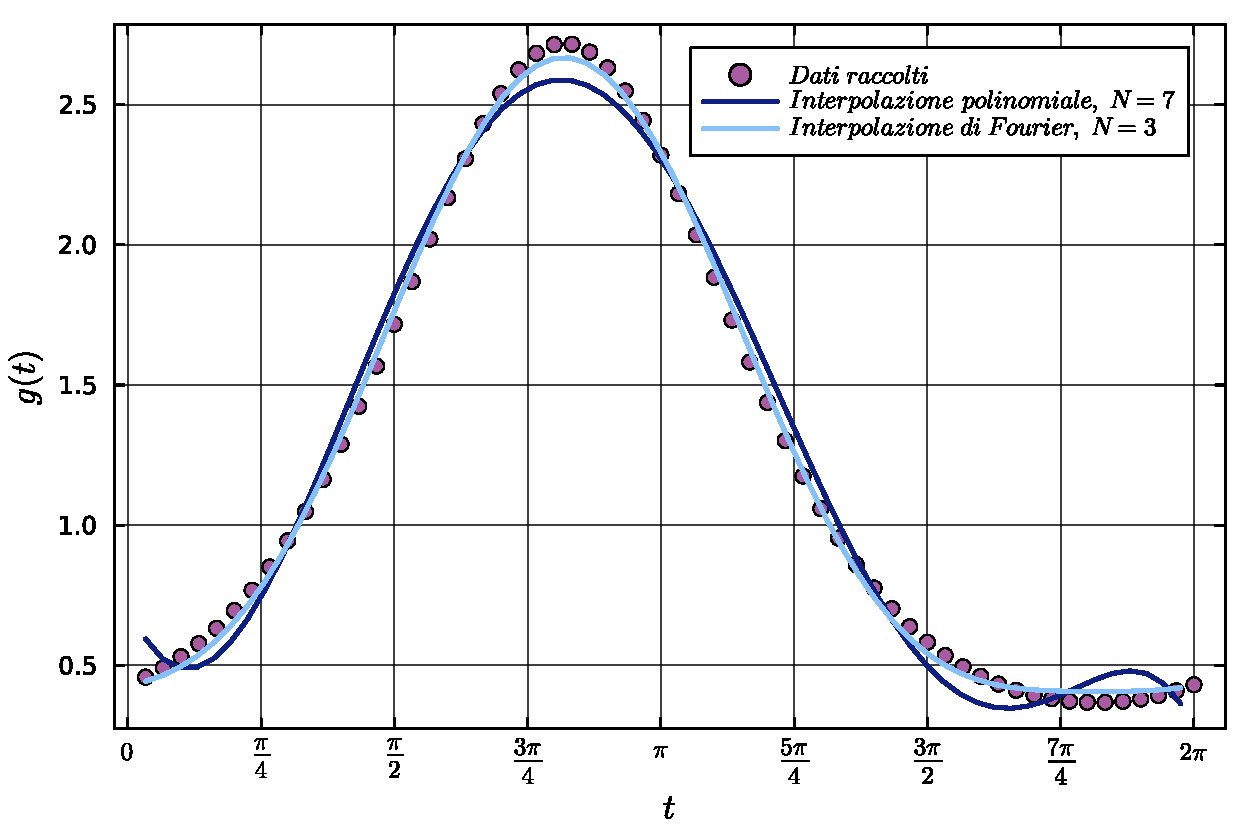
\includegraphics[width=0.8\textwidth]{2631.pdf}
    \caption{Fit polinomiale e di Fourier ai minimi quadrati della funzione $g(t)=e^{\sin(t-1)}$.}
    \label{fig:es2_6_3_1}
\end{figure}

\subsubsection{Conclusioni}
In figura \ref{fig:es2_6_3_1} si osserva che il fit meglio riuscito è quello di Fourier, nonostante
richieda meno parametri. Il motivo è che la funzione $g(t)$ è periodica, e quindi il fit con il modello 
\ref{eq:fit_fourier} riesce a catturare meglio la periodicità della funzione rispetto al fit esguito con 
\ref{eq:fit_pol}. \\
In un contesto sperimentale la funzione $g(t)$ non è nota a priori, anzi lo scopo dell'esperimento è 
solitamente quello di risalire a tale funzione. Il fatto che il fit secondo il modello di Fourier riesca meglio
è indice della natura periodica del fenomeno osservato. 

\section{Radici di equazioni non lineari}
\subsection{Teoria}

\subsection{Esercizi 3.2.1, 3.2.2}
1. Implementa il metodo di bisezione e testalo con una funzione semplice, ad esempio $f(x)=x$. \\
2. (a) Usa il metodo di bisezione per trovare le soluzioni di $x^3 - 7x^2 + 14x - 6 = 0$ su $[0,1]$.\\
   (b) Studia la convergenza del metodo di bisezione rispetto alla radice trovata in (a). 
   (Puoi prendere come approssimazione per la radice $r=m_{n_{\rm max}}$, dove $n_{\rm max}$ è 
   l'indice corrispondente all'ultima iterazione di bisezione.) \\
   Qual è il suo ordine di convergenza $q$? Puoi stimare la costante d'errore asintotica $C$? \\
   Suggerimento: Studia $d_n=-\log_{10}|x_{n}-r|$ come funzione di $n$.

%Riguarda i conti teorici. Sono giusti ma vanno formalizzati
\subsubsection{Soluzione}
\paragraph{(1) } Si è implementato il metodo di bisezione, e si è testato con la funzione $f(x)=x$ per due 
intervalli: $[-1.0, 1.0]$ e $[-5.0, 1.0]$. Il motivo della scelta di questi due intervalli è che ci aspettiamo che
il metodo restituisca $x = 0$ come soluzione e nel caso di intervallo simmetrico il numero di iterazioni 
è pari ad 1. Con un intervallo asimmetrico il test è più efficiente perchè il numero di iterazioni aumenta. \\
Il metodo si interrompe quando la distanza tra gli estremi risulta minore di $\max(|a|,|b|) \cdot 10^{-16}$,
dove $a$ e $b$ sono gli estremi dell'intervallo. Il metodo ha prodotto i seguenti risultati:
\begin{itemize}
    \item Intervallo $[-1.0, 1.0]$: $x = 0.0$ in 1 iterazione.
    \item Intervallo $[-5.0, 1.0]$: $x = 1.1 \cdot 10^{-162}$ in 539 iterazioni.
\end{itemize}

\paragraph{(2a) } Si è implementato il metodo di bisezione per la funzione $f(x) = x^3 - 7x^2 + 14x - 6$. \\
Il metodo ha restituito un valore della radice $r = 0.5857864376269051$ con $f(r) = 0.0$, in $50$ iterazioni. In
figura \ref{fig:es3_2_2_1} si riporta il grafico della funzione e delle radici successive trovate.
\begin{figure}
    \centering
    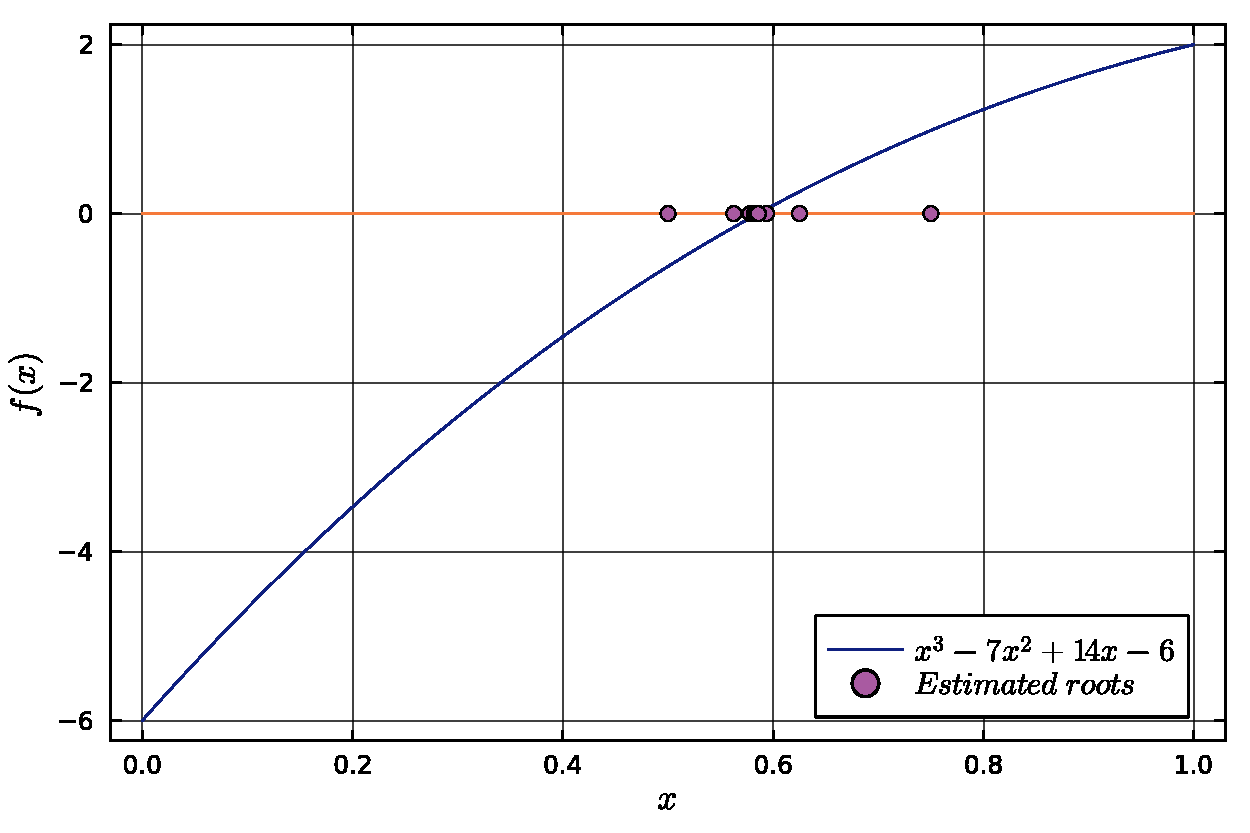
\includegraphics[width=0.8\textwidth]{3221.pdf}
    \caption{Grafico della funzione $f(x) = x^3 - 7x^2 + 14x - 6$ e della radice trovata con il metodo di bisezione.}
    \label{fig:es3_2_2_1}
\end{figure} 

\paragraph{(2b) } Per studiare la convergenza del metodo di bisezione bisogna fare alcune considerazioni 
preliminari. \\
È noto che per il metodo di bisezione vale la relazione $ |m_n-r|< 2^{-(n+1)} (b_0-a_0) $, dove $m_n$ è 
la stima della radice al passo $n$, $r$ è la radice cercata, $a_0$ e $b_0$ sono gli estremi dell'intervallo 
iniziale. \\
Ad ogni iterazione l'intervallo viene dimezzato, in modo che al passo successivo la stima della radice si trovi
in una delle due metà dell'intervallo nella quale si trovava la stima precedente. In formule: 
$|m_{n+1}-r| <\frac{|m_n-r|}{2}$. \\
Unendo le due relazioni presentate sopra si ricava $\frac{|m_{n+1}-r|}{|m_n-r|} < \frac{1}{2}$, e passando al 
limite: 
\begin{equation}
    \label{eq:convergenza_bisezione}
    \lim_{n\to\infty} \frac{|m_{n+1}-r|}{|m_n-r|} = \frac{1}{2}, 
\end{equation}
da cui si ottiene che $q$, ordine di convergenza, 
è 1, mentre C, la costante di errore asintotico, vale $\frac{1}{2}$. \\
Verifichiamolo numericamente, ricordando le relazioni: 

Per verificare i valori teorici di $q$ e $C$ è necessario tenere a mente le seguenti relazioni. La prima si ottiene
applicando il logaritmo decimale alla \ref{eq:convergenza_bisezione}:
\begin{equation}
    \label{eq:convergenza_bisezione_log}
    d_{n+1} \approx q\, d_n - \log_{10}|C|
    \quad\Rightarrow\quad
    \frac{d_{n+1}}{d_n} \approx q - \frac{\log_{10}|C|}{d_n}
    \overset{n\to\infty}{\longrightarrow} q
\end{equation}

dove $d_n = -\log_{10}|m_n - r|$. \\
La seconda si ottiene iterando la relazione  $ |x_{k+1} - r|= C |x_{k} - r|$:
\begin{equation}
    |x_{k+1} - r|= C^{k+1} |x_{0} - r|
\end{equation}

\subparagraph{Stima di $q$} Per stimare $q$ si è calcolato il rapporto tra i valori di $d_n$ e $d_{n+1}$ e lo si
è messo in grafico in funzione di $n$, ottenendo la figura \ref{fig:es3_2_2_2}, in cui è presente un ingrandimento
per i valori più alti di n.
\begin{figure}[!ht]
    \centering
    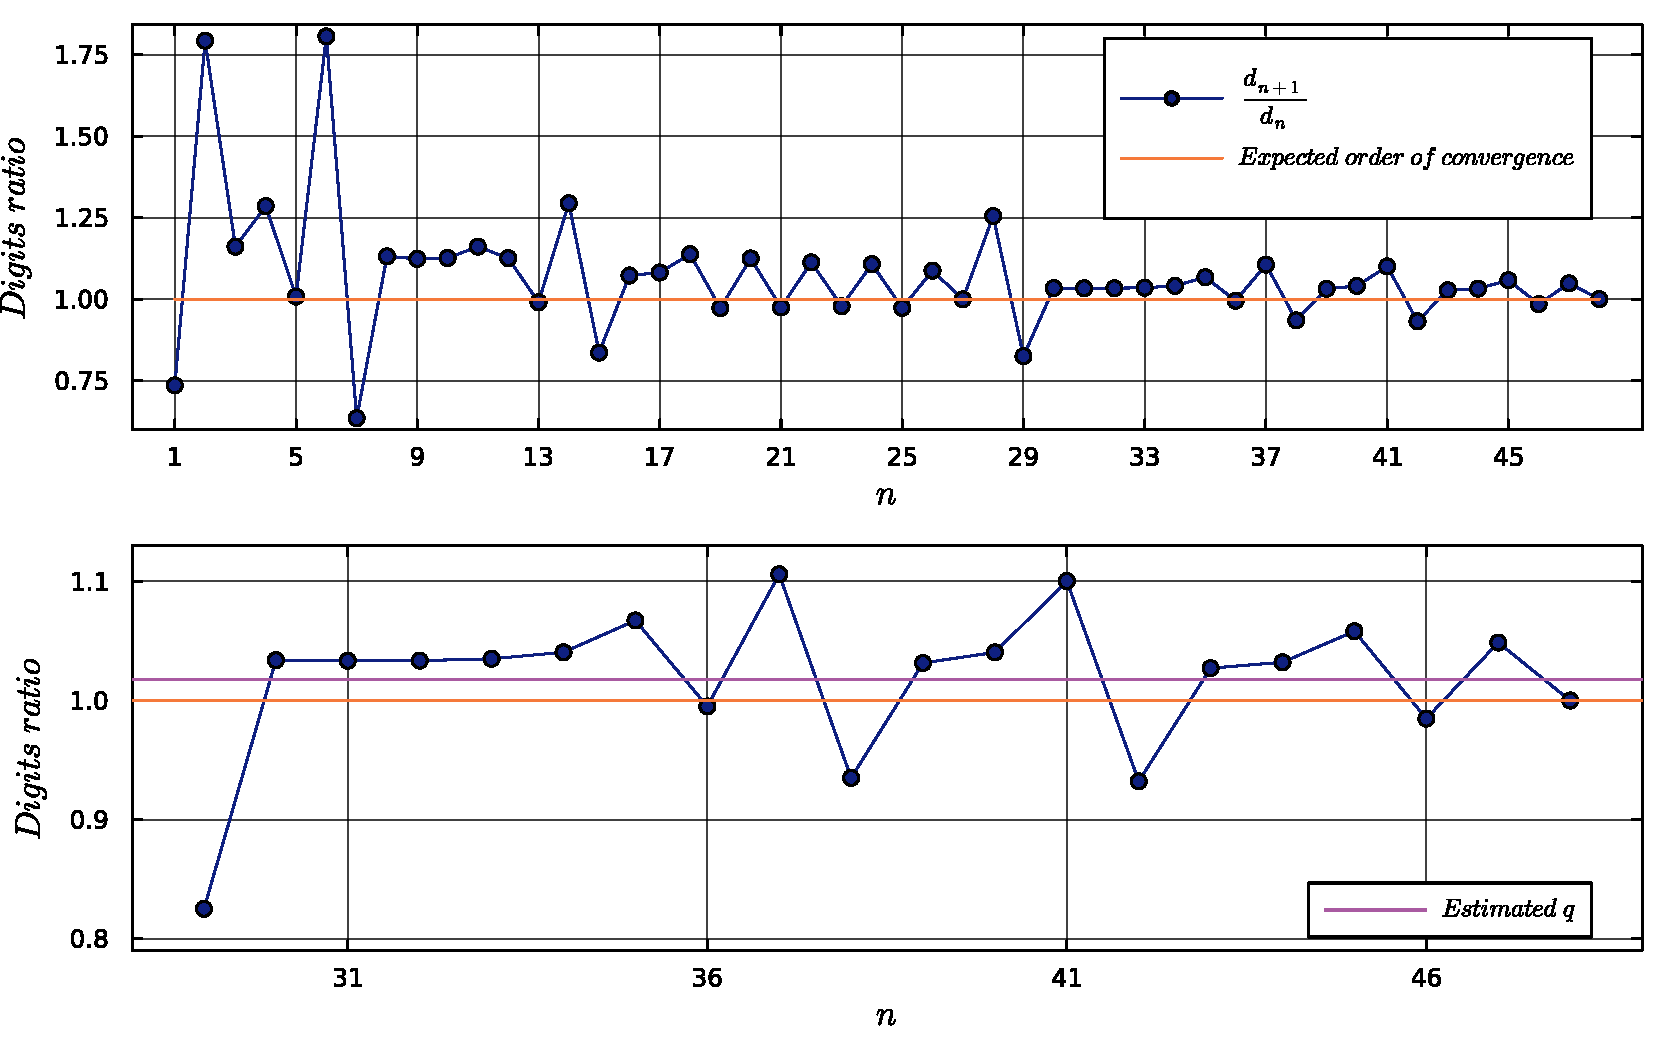
\includegraphics[width=0.8\textwidth]{3222.pdf}
    \caption{Rapporto tra i valori di $d_n$ e $d_{n+1}$ in funzione di $n$.}
    \label{fig:es3_2_2_2}
\end{figure}

Il rapporto tende a 1, come atteso. Si vuole ora quantificare tale valore. \\
La relazione \ref{eq:convergenza_bisezione_log} vale per $n\to\infty$. Ciò significa che la stima di $q$
dovrebbe essere calcolata per l'$n$ più grande possibile. Ciononostante si
è deciso di stimare il valore di $q$ tramite l'interpolazione con funzione costante perchè il valore di $q$ 
fluttua attorno a 1, ed è possibile che per $n$ maggiori di quelli disponibili il valore cercato continui a 
fluttuare attorno a 1. Per l'interpolazione si sono considerati gli ultimi 20 punti della serie, riportati 
nell'ingrandimento di \ref{fig:es3_2_2_2}. Il fit su tali punti restituisce
un valore di $q = 1.02$. \\  

\subparagraph{Stima di $C$}
Per stimare $C$ si è eseguito il fit con metodo dei minimi quadrati sul modello:
\begin{equation}
    log |x_{k+1}-r| = (k+1)log(C) + log|x_0 - r|   \rightarrow   y(x) = x log(C) + A ,
\end{equation}
avendo considerato $r$ come l'ultimo valore di $m_n$ calcolato. Si riporta il grafico del fit in figura \ref{fig:es3_2_2_3}.
\begin{figure}[!ht]
    \centering
    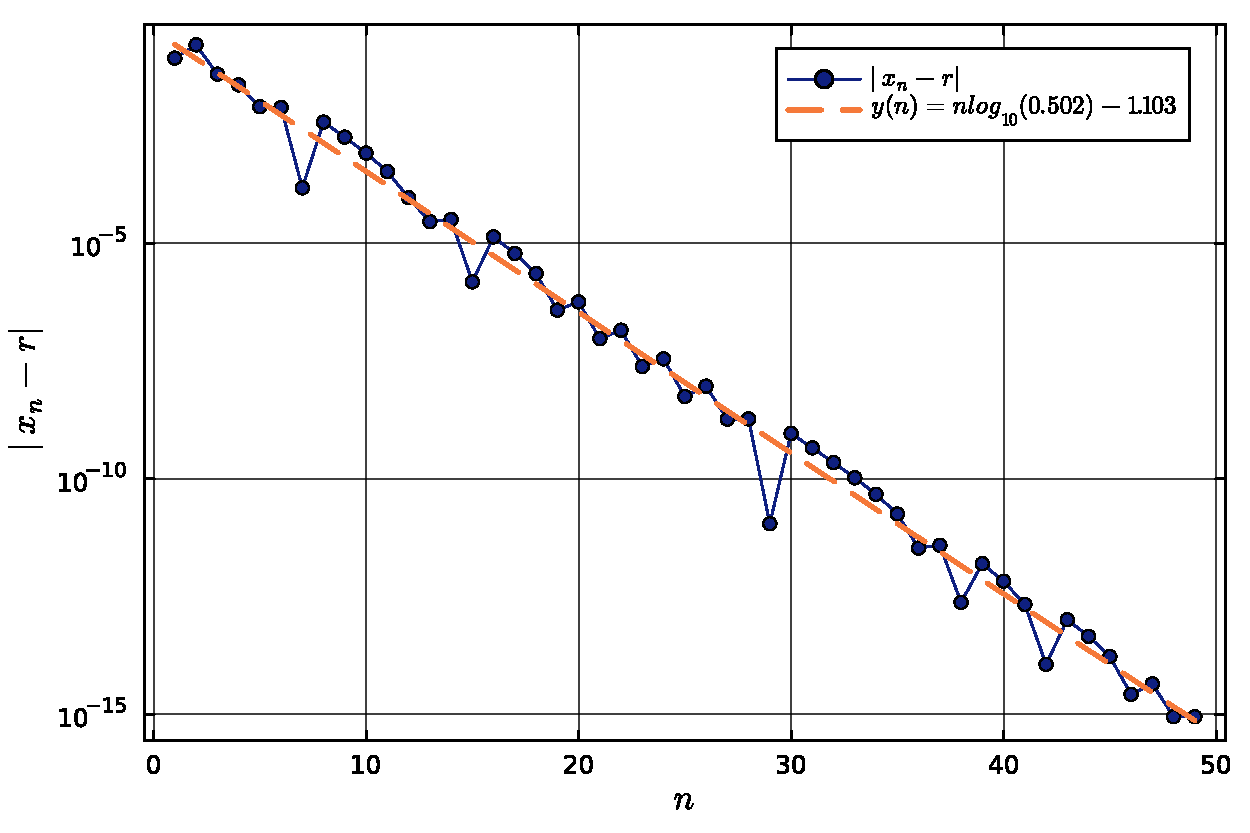
\includegraphics[width=0.8\textwidth]{3223.pdf}
    \caption{Fit lineare del logaritmo decimale della distanza tra la radice e le stime successive.}
    \label{fig:es3_2_2_3}
\end{figure}
Il fit ha restituito i seguenti valori:
\begin{equation}
    C = 0.5 \pm 0.01,
    \qquad
    A = -0.1 \pm 0.01.
\end{equation}
Si osserva che il valore di $C$ è in accordo con quanto atteso, mentre il valore di $A$ non è significativo.

\subparagraph{Commento: } È possibile stimare i valori di $q$ e $C$ anche in modo diverso, e con un solo fit.
Interpolando la relazione \ref{eq:convergenza_bisezione_log} con un'iperbole, e ignorando il limite, 
si riescono a ottenere i valori di $q$ e $C$ in un colpo solo. I risultati ottenuti hanno una precisione minore 
di quelli ottenuti  con i metodi precedenti, pertanto non sono riportati. Si rimanda alla cartella git
\verb|lab\computazionale1\esercizi\3_2_2.ipynb| per i dettagli.

\section{Interpolazioni}
\subsection{Teoria}

\section{Integrazione numerica}
\subsection{Teoria}

\section{Equazioni differenziali ordinarie}
\subsection{Teoria}

\section{Appendice}
\subsection{Dati}

\begin{table}[!ht]
    \centering
    \caption{Distanza dal Sole e periodo orbitale dei pianeti del Sistema Solare}
    \label{tab:pianeti}
        \begin{tabular}{|l|c|c|}
        \hline
        \textbf{Pianeta} & \textbf{Distanza dal Sole [Mkm]} & \textbf{Periodo orbitale [giorni]} \\
        \hline
        Mercurio & 57.59   & 87.99   \\
        Venere   & 108.11  & 224.7   \\
        Terra    & 149.57  & 365.26  \\
        Marte    & 227.84  & 686.98  \\
        Giove    & 778.14  & 4332.4  \\
        Saturno  & 1427    & 10759   \\
        Urano    & 2870.3  & 30684   \\
        Nettuno  & 4499.9  & 60188   \\
        \hline
        \end{tabular}
\end{table}
\end{document}